% ============================================================================
% g-BKMR Application Paper — Strong Heart Study
% Lead: Arce Domingo-Relloso
% Yanran Li writes the Application (Results) section
% Target: Environmental Health (Springer/BMC) — same venue as Bobb et al. 2018
% ============================================================================
\documentclass[11pt]{article}

\usepackage[utf8]{inputenc}
\usepackage[T1]{fontenc}
\usepackage{lmodern}
\usepackage[a4paper,margin=1in]{geometry}
\usepackage{amsmath,amssymb}
\usepackage{graphicx}
\usepackage{booktabs}
\usepackage{caption}
\usepackage{subcaption}
\usepackage{hyperref}
\usepackage[round]{natbib}
\usepackage{authblk}
\usepackage{lineno}
\usepackage{xcolor}
\usepackage{setspace}

\hypersetup{colorlinks=true, linkcolor=blue!60!black, citecolor=blue!60!black, urlcolor=blue!60!black}

\newcommand{\todo}[1]{{\color{red}\textbf{[TODO: #1]}}}
\newcommand{\note}[1]{{\color{purple}\textit{[#1]}}}

\linenumbers
\onehalfspacing

% --- Title and authors (from gBKMR_Nature.docx) ----------------------------
\title{g-BKMR: Causal Inference for Health Effects of Time-varying Correlated Environmental Mixtures}

\author[1]{Zilan Chai}
\author[1]{Arce Domingo-Relloso}
\author[1]{Yanran Li}
\author[2]{Ana Navas-Acien}
\author[3]{Brent A.\ Coull}
\author[1,4]{Linda Valeri}

\affil[1]{Department of Biostatistics, Columbia University Mailman School of Public Health, New York, NY, USA}
\affil[2]{Department of Environmental Health Sciences, Columbia University Mailman School of Public Health, New York, NY, USA}
\affil[3]{Department of Biostatistics, Harvard T.H.\ Chan School of Public Health, Boston, MA, USA}
\affil[4]{Department of Epidemiology, Harvard T.H.\ Chan School of Public Health, Boston, MA, USA}

\date{\today}

\begin{document}
\maketitle

% ============================================================================
% ABSTRACT (BMC structured: Background / Methods / Results / Conclusions)
% ============================================================================
\begin{abstract}
\noindent\textbf{Background.} \todo{Arce + Linda. From gBKMR\_Nature.docx.}

\noindent\textbf{Methods.} \todo{Arce + Linda.}

\noindent\textbf{Results.} \todo{Arce + Linda + Yanran.}

\noindent\textbf{Conclusions.} \todo{Arce + Linda.}
\end{abstract}

% ============================================================================
% INTRODUCTION
% ============================================================================
\section{Introduction}
\label{sec:intro}

\note{Arce + Linda. Migrate from gBKMR\_Nature.docx Introduction section.}

\todo{Environmental mixtures, time-varying confounding, gap, g-BKMR contribution, SHS application.}

% ============================================================================
% METHODS
% ============================================================================
\section{Methods}
\label{sec:methods}

\note{Arce + Linda. Migrate from gBKMR\_Nature.docx Methods section.}

\subsection{Identifiability assumptions and estimation}
\todo{g-formula, consistency, sequential exchangeability, positivity.}

\subsection{Bayesian Kernel Machine Regression}
\todo{BKMR review, Gaussian kernel, variable selection.}

\subsection{g-BKMR}
\todo{Algorithm combining g-formula with BKMR.}

% ============================================================================
% RESULTS
% ============================================================================
\section{Results}
\label{sec:results}

\subsection{Simulation study}
\label{sec:simulation}

\note{Arce + Linda. Existing simulation results.}

\todo{Simulation design, comparison with alternatives, coverage/bias results.}

% ---------- APPLICATION SECTION (Yanran) ----------

\subsection{Application: metal mixture exposure and fasting blood glucose in the Strong Heart Study}
\label{sec:application}

\subsubsection{Study population and exposures}

We applied g-BKMR to data from the Strong Heart Study (SHS), a prospective cohort of American Indian adults with low to moderate exposure to metals and a high burden of cardiometabolic disease. The analytic sample consisted of 679 participants with complete urinary metal measurements at three study visits (Visits 1--3) and fasting blood glucose measured at Visit 3. Six urinary metals were considered: selenium (Se), cadmium (Cd), molybdenum (Mo), tungsten (W), arsenic (As), and zinc (Zn), all standardised to urinary creatinine and log-transformed prior to analysis. The mixture comprised 18 exposure variables (six metals $\times$ three visits).

The outcome was log-transformed fasting blood glucose at Visit~3 (motivated by right-skewed distributions; skewness $1.8$--$2.1$; see Supplementary Figure~\ref{fig:supp-dist}). Time-varying confounders included waist circumference and fasting glucose measured at Visits 1 and 2, modeled as time-dependent covariates affected by prior exposure. Baseline covariates included age, sex, body mass index, study centre, smoking status (current/former/never), and baseline kidney function (CKD-EPI eGFR). Missing values were handled by multiple imputation ($m = 5$, predictive mean matching). The directed acyclic graph encoding the assumed causal structure is shown in Figure~\ref{fig:dag}; the cross-timepoint correlation matrix is shown in Figure~\ref{fig:corr}.

\subsubsection{Model specification and estimation}

We fit g-BKMR with component-wise variable selection. For each multiply imputed dataset, the BKMR mediator and outcome models were fit using $24{,}000$ MCMC iterations with the final $2{,}000$ retained for posterior summaries (every 50th draw). We targeted two estimands: (i) the joint mixture causal effect, defined as the average causal effect of jointly shifting all 18 metal-timepoint exposures from their 25th percentile (reference) to a target percentile $q \in \{0.30, 0.35, \ldots, 0.90\}$, and (ii) single-variable causal effects, defined as the effect of shifting one metal at one visit from its 25th to 75th percentile while holding all other exposures at their 50th percentile. Posterior means and 95\% credible intervals (CrIs) were obtained by pooling MCMC draws across the five imputed datasets.

\subsubsection{Joint mixture effect}

The joint mixture causal effect on log fasting glucose followed a positive, approximately monotonic dose-response (Figure~\ref{fig:dr-joint}). The 95\% credible interval excluded zero above approximately the 45th percentile, with the magnitude of the effect increasing through the upper end of the exposure distribution. At the 75th vs.\ 25th percentile contrast, the average causal effect was $1.01$ standardised units of log glucose (95\% CrI: $0.72$, $1.33$).

\subsubsection{Single-variable effects}

Examining each metal-timepoint individually (Figure~\ref{fig:forest}), zinc was the dominant contributor to the joint mixture signal: the IQR causal effect of Zn was $0.51$ SD at Visit~1 (95\% CrI: $0.28$, $0.75$), $0.26$ SD at Visit~2 ($0.03$, $0.51$), and $0.36$ SD at Visit~3 ($0.20$, $0.55$). All three Zn-timepoint effects were credibly distinct from zero. Selenium at Visit~1 also showed a positive association ($0.19$ SD; 95\% CrI: $-0.01$, $0.36$; posterior probability of a positive effect: $0.97$). Cadmium at Visit~1 showed an inverse association ($-0.21$ SD; 95\% CrI: $-0.37$, $-0.05$). The remaining metal-timepoints (Mo, W, As, and the later visits of Se and Cd) had effect estimates with credible intervals overlapping zero. Per-metal dose-response curves are shown in Supplementary Figure~\ref{fig:supp-permetal}.

\subsubsection{Sensitivity to baseline diabetes status}

Because metals may differentially affect glucose metabolism in individuals with established diabetes, we conducted a sensitivity analysis excluding the 265 participants with baseline diabetes (WHO clinical definition; analytic sample $n = 414$). In this subsample, the joint mixture dose-response was substantially attenuated, with the 95\% credible interval covering zero across most quantile contrasts (Figure~\ref{fig:dr-compare}). Single-variable effects were also markedly reduced (Supplementary Figure~\ref{fig:supp-forest-nodm}): Zn(V1) decreased from $0.51$ to $0.01$ SD, Cd(V1) reversed sign and became non-significant, and most other estimates moved toward the null. Two findings remained robust: Se(V1) remained positive and credibly above zero ($0.07$ SD; 95\% CrI: $0.004$, $0.15$), and Zn(V3) retained a borderline positive signal ($0.14$ SD; 95\% CrI: $0.00$, $0.35$).

\subsubsection{Sensitivity to smoking intensity}

To address potential residual confounding by smoking intensity---particularly relevant to the inverse Cd(V1) finding---we additionally adjusted for baseline pack-years alongside the categorical smoking-status variable. For never-smokers, pack-years was set to zero prior to multiple imputation. All findings were robust to this adjustment (Supplementary Table~\ref{tab:supp-packyears} and Supplementary Figure~\ref{fig:supp-forest-ppy}): the joint dose-response at the 75th vs.\ 25th percentile was $1.06$ SD (95\% CrI: $0.80$, $1.39$), compared with $1.01$ ($0.72$, $1.33$) in the main analysis. Notably, the inverse Cd(V1) effect was essentially unchanged ($-0.22$ SD; 95\% CrI: $-0.35$, $-0.10$), indicating that this association is not explained by smoking intensity alone.

% ============================================================================
% DISCUSSION
% ============================================================================
\section{Discussion}
\label{sec:discussion}

\note{Arce + Linda. Key discussion points from meetings:}

\todo{(a) Se(V1): robust, independent of baseline DM, consistent with SELECT trial.}

\todo{(b) Cd(V1): inverse, not explained by pack-years, V1-only pattern needs interpretation.}

\todo{(c) Zn--glucose: attenuated after excluding DM; measurement confounding from imperfectly captured prior glucose/zinc trajectories rather than reverse causation. Cite Linda + Irene under-review longitudinal mediation paper.}

\todo{(d) Strengths and limitations of g-BKMR and the SHS data.}

% ============================================================================
% CONCLUSIONS
% ============================================================================
\section{Conclusions}
\label{sec:conclusions}

\note{Arce + Linda.}

\todo{Summary paragraph.}

% ============================================================================
% DECLARATIONS
% ============================================================================
\section*{Declarations}

\subsection*{Funding}
\todo{Grant numbers.}

\subsection*{Availability of data and materials}
Strong Heart Study data are available from the SHS Coordinating Center upon request and after approval by the participating American Indian tribes. Code for the g-BKMR analysis is available at \todo{GitHub URL}.

\subsection*{Ethics approval and consent to participate}
The Strong Heart Study was approved by the Indian Health Service Institutional Review Board, the institutional review boards of the participating American Indian tribes, and the institutional review boards of the participating institutions. All participants provided written informed consent.

\subsection*{Authors' contributions}
\todo{Author contributions.}

\subsection*{Competing interests}
The authors declare no competing interests.

\subsection*{Acknowledgements}
\todo{Tribes, study staff, funding.}

% ============================================================================
% REFERENCES
% ============================================================================
\bibliographystyle{plainnat}
\bibliography{references}

% ============================================================================
% FIGURES
% ============================================================================
\clearpage
\section*{Figures}

\begin{figure}[h]
\centering
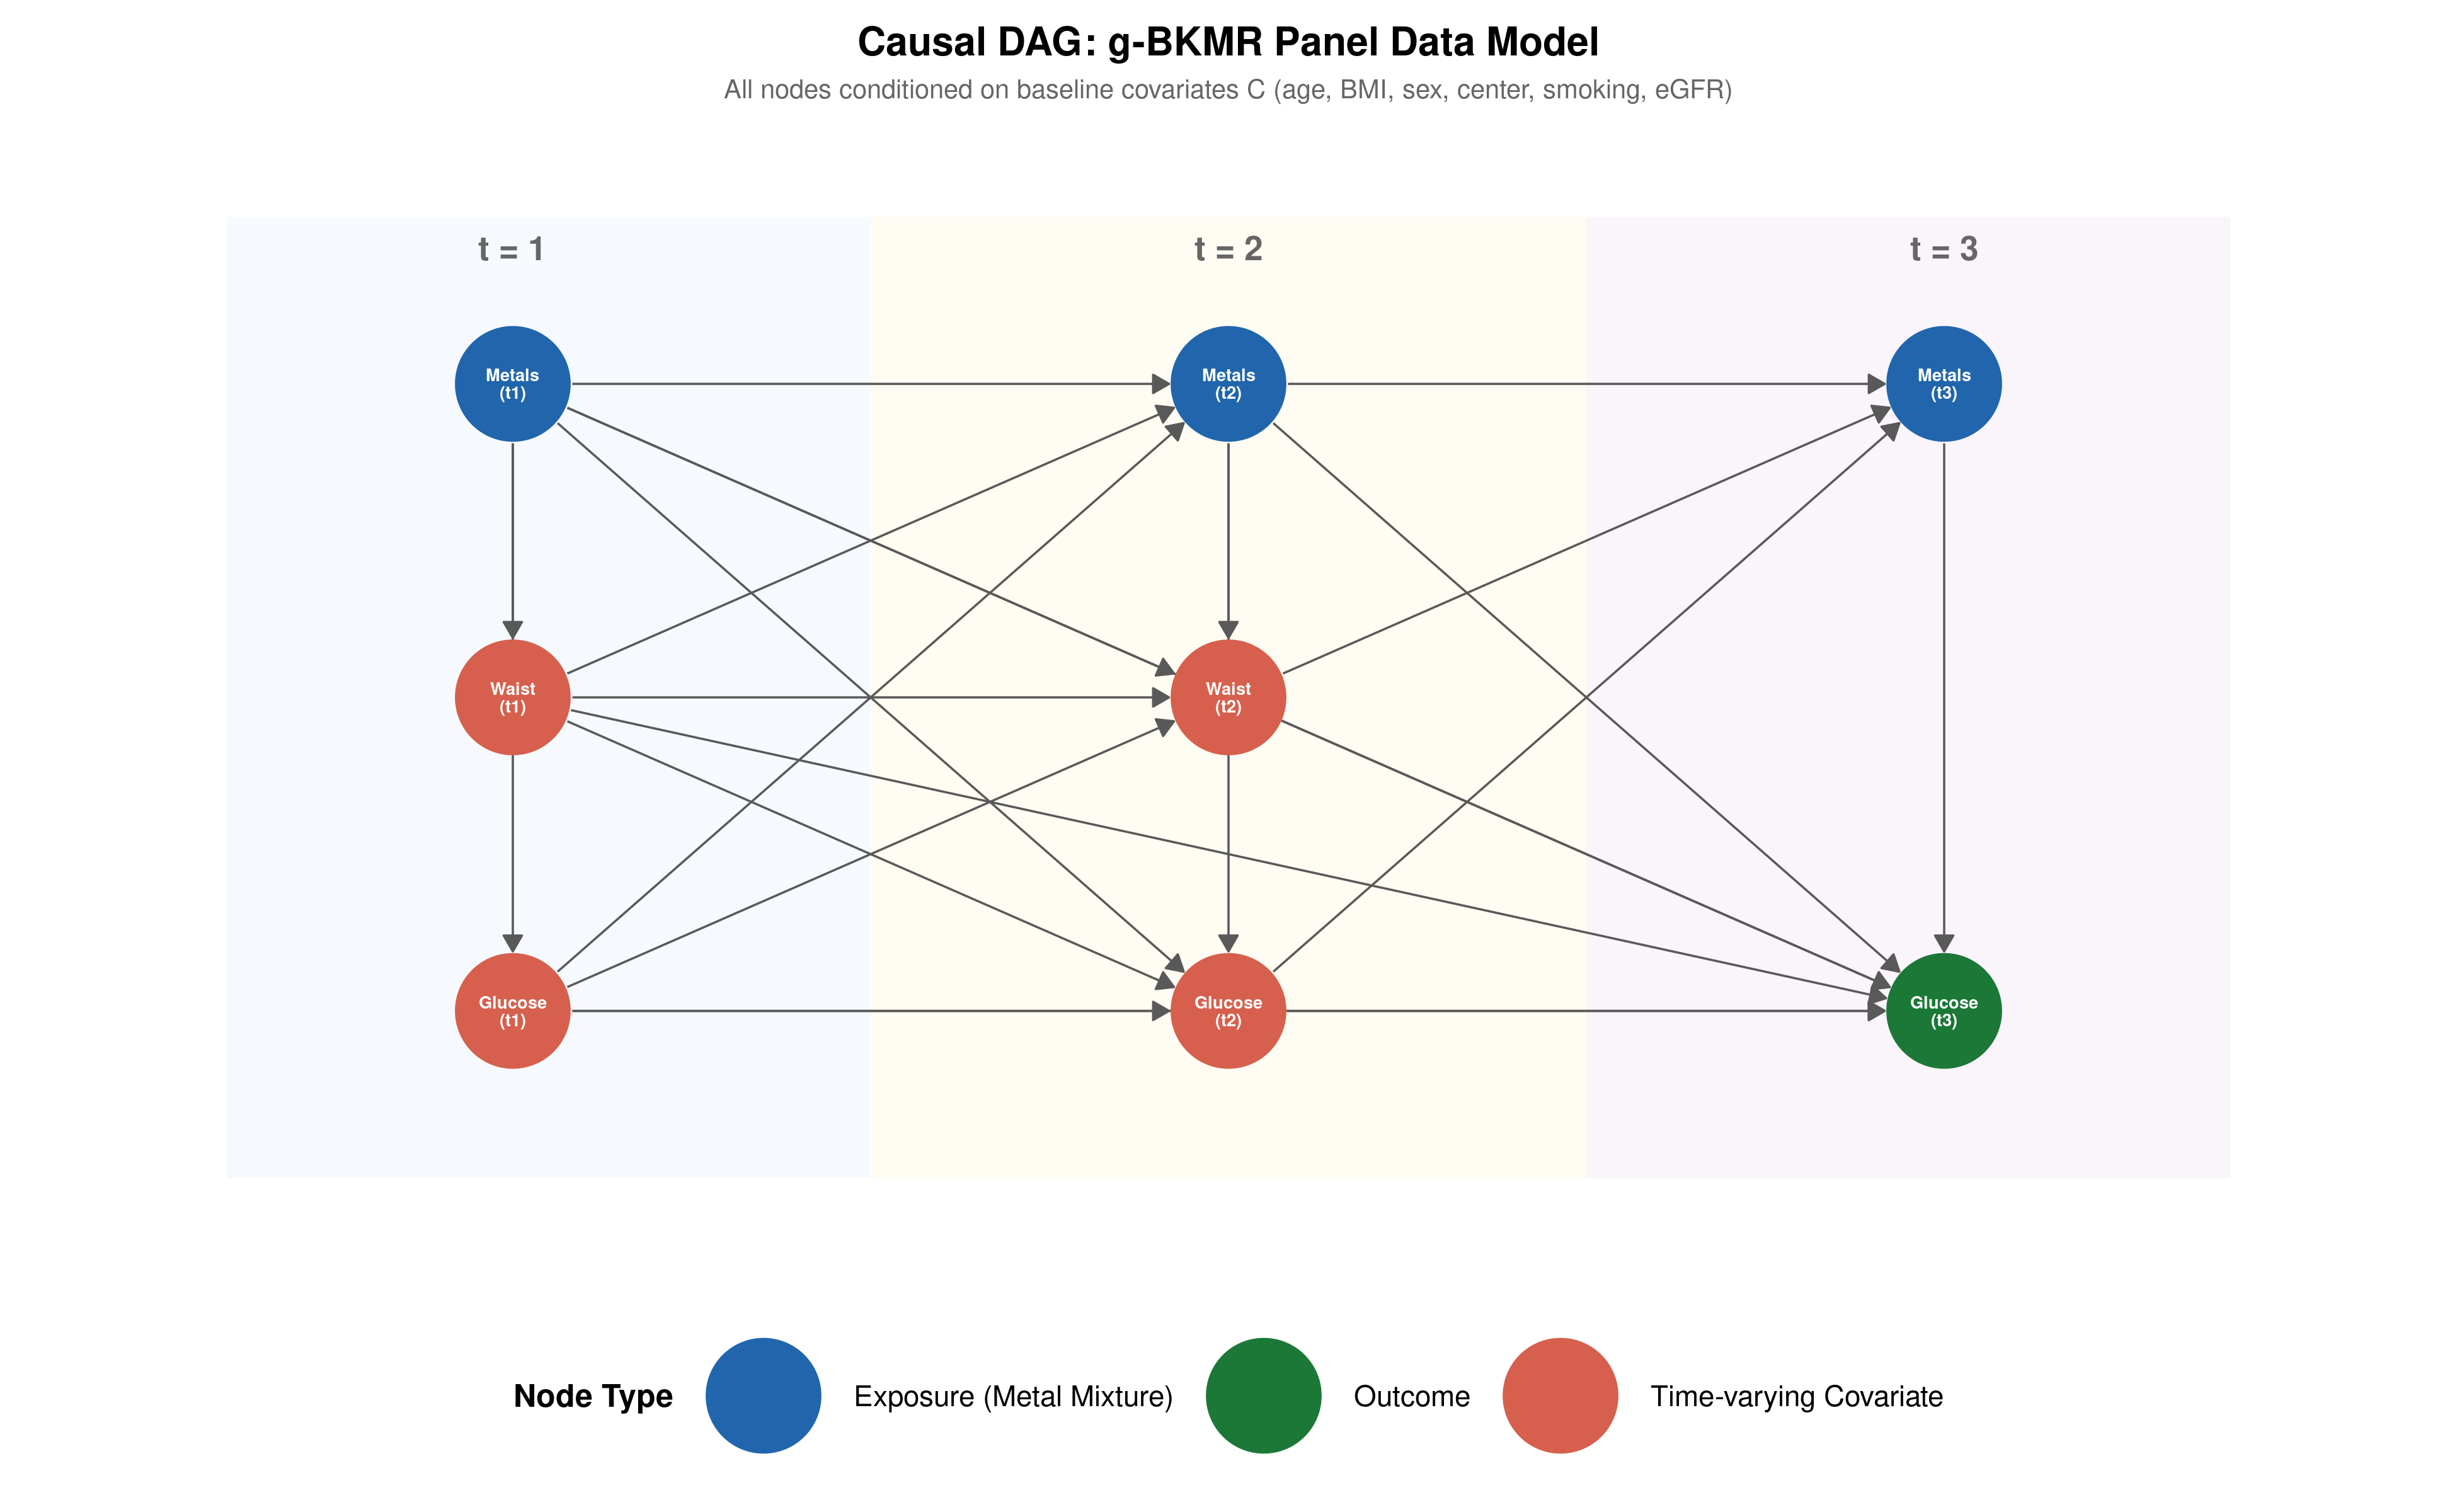
\includegraphics[width=0.7\textwidth]{figures/fig_dag.png}
\caption{Directed acyclic graph for the Strong Heart Study application.}
\label{fig:dag}
\end{figure}

\begin{figure}[h]
\centering
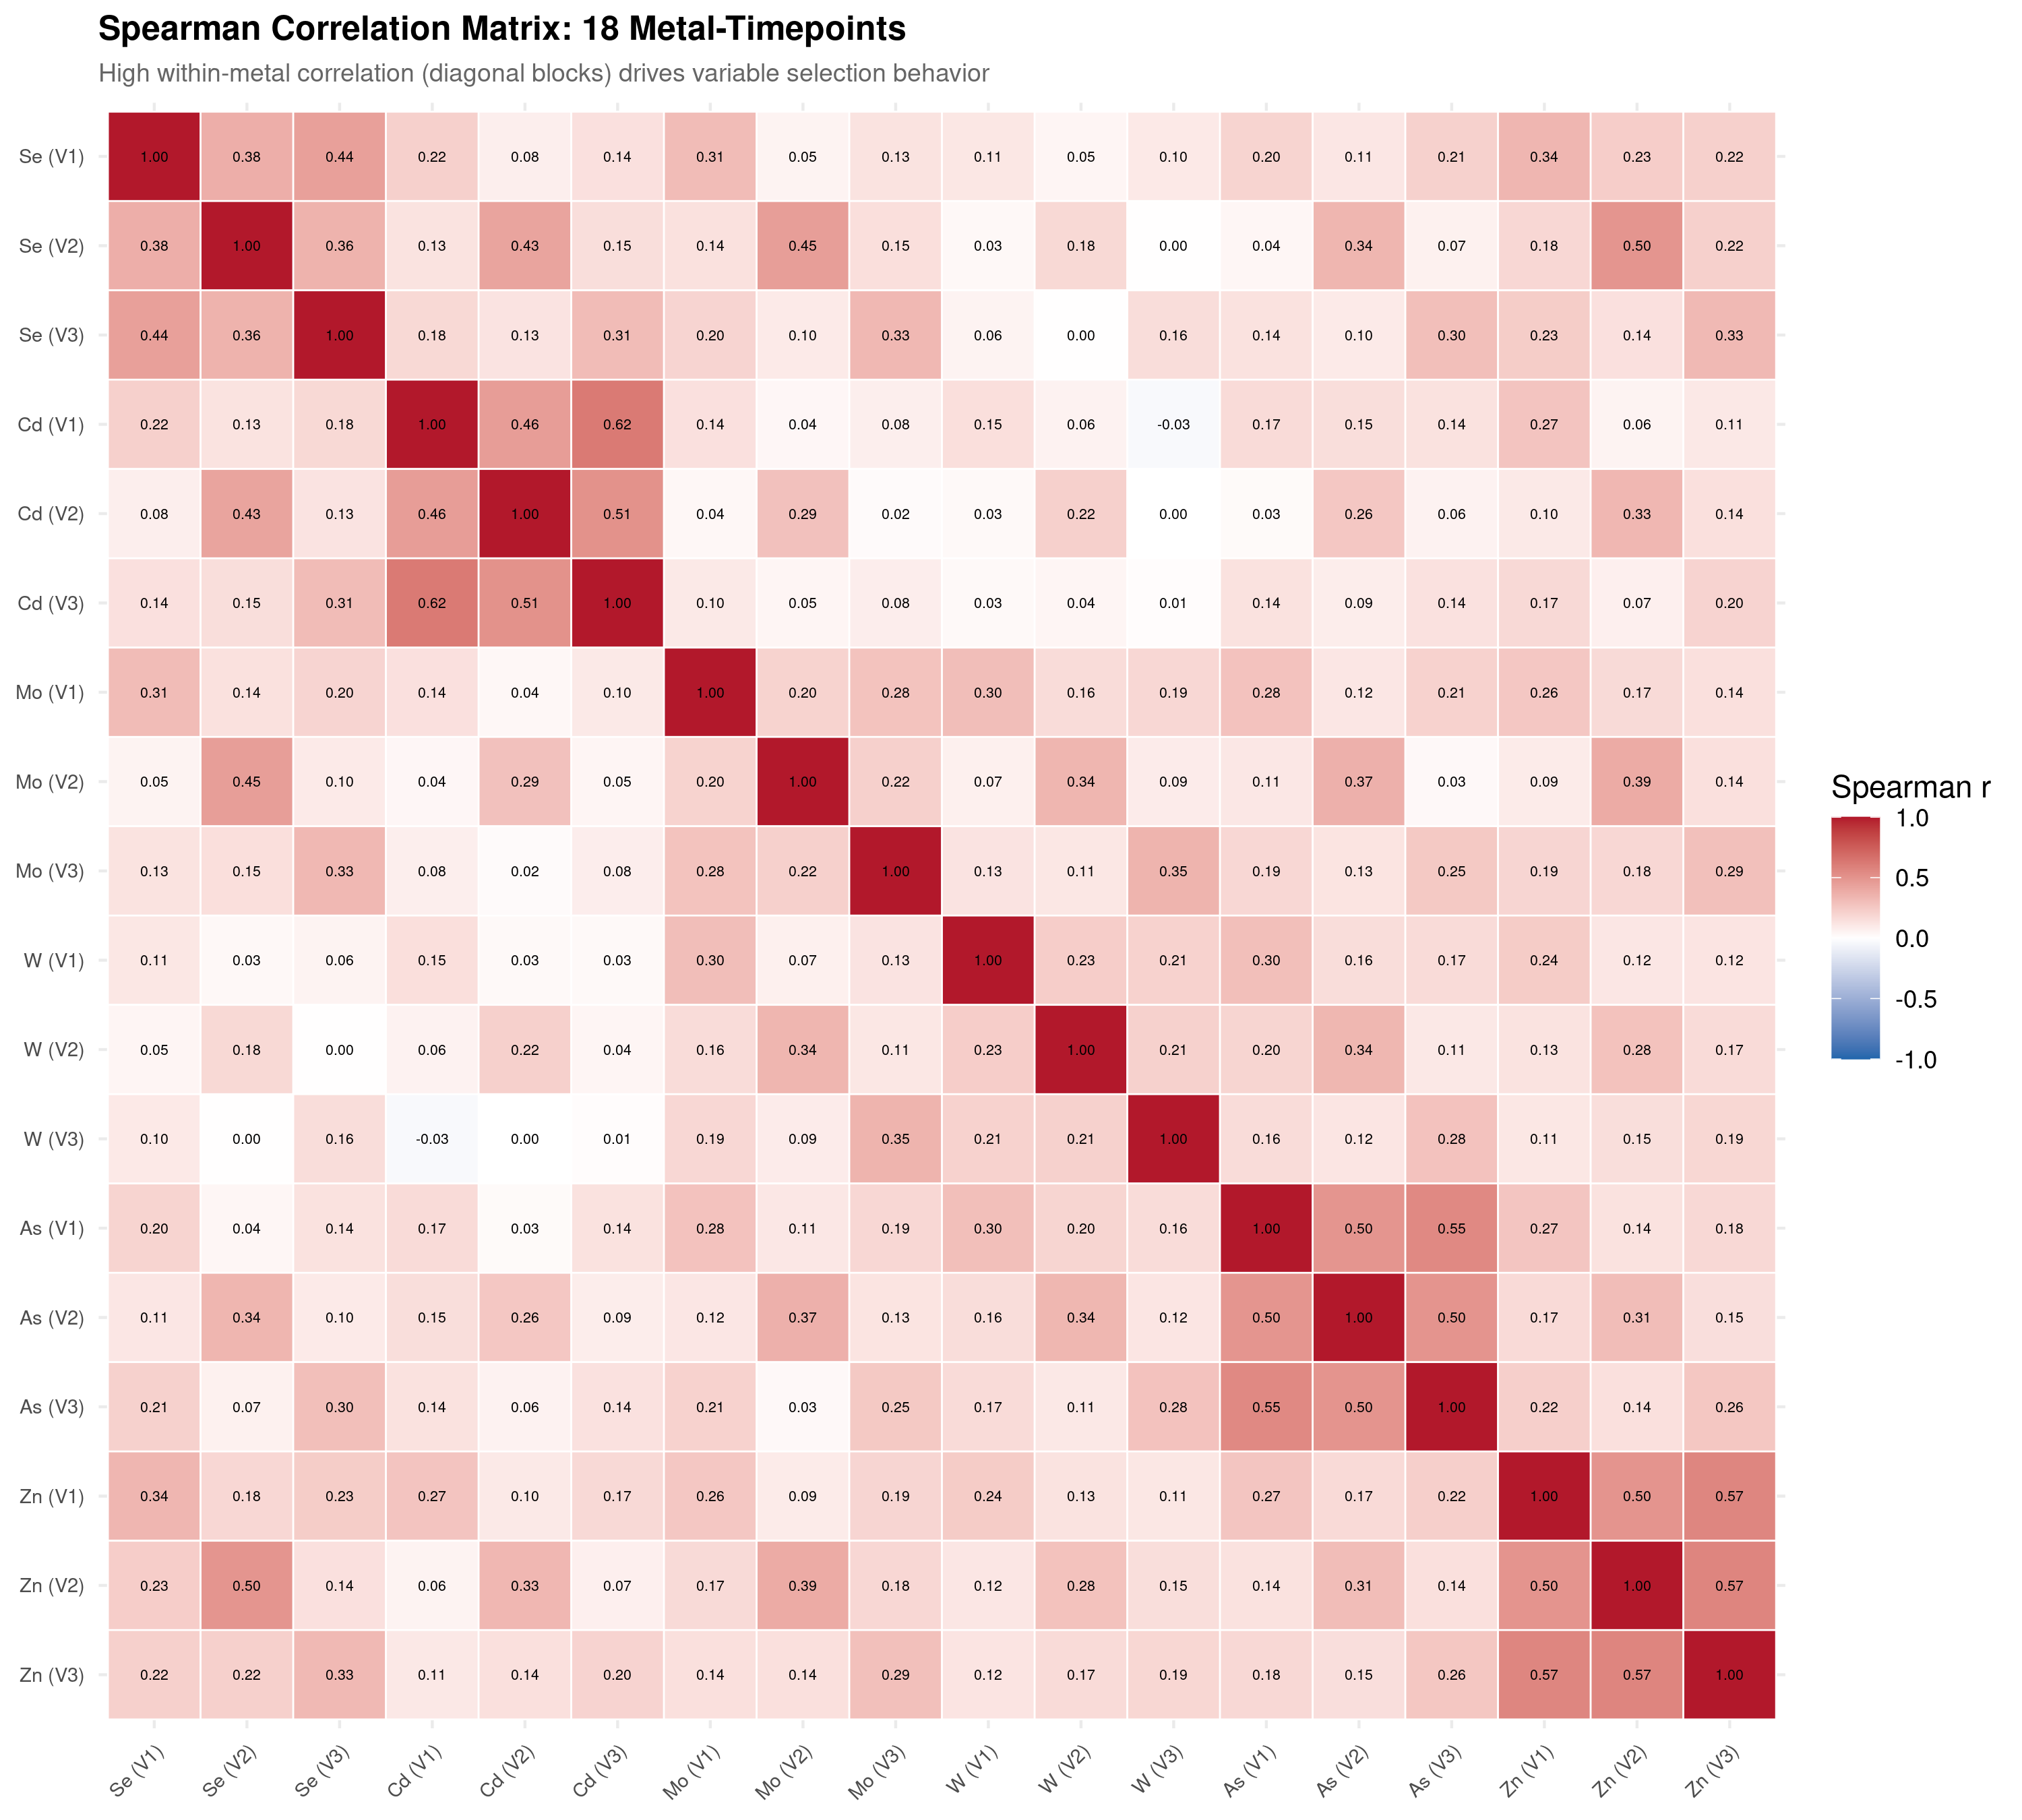
\includegraphics[width=0.85\textwidth]{figures/fig_cross_timepoint_corr_matrix.png}
\caption{Spearman correlation matrix of the 18 metal-timepoint exposures (six metals $\times$ three visits).}
\label{fig:corr}
\end{figure}

\begin{figure}[h]
\centering
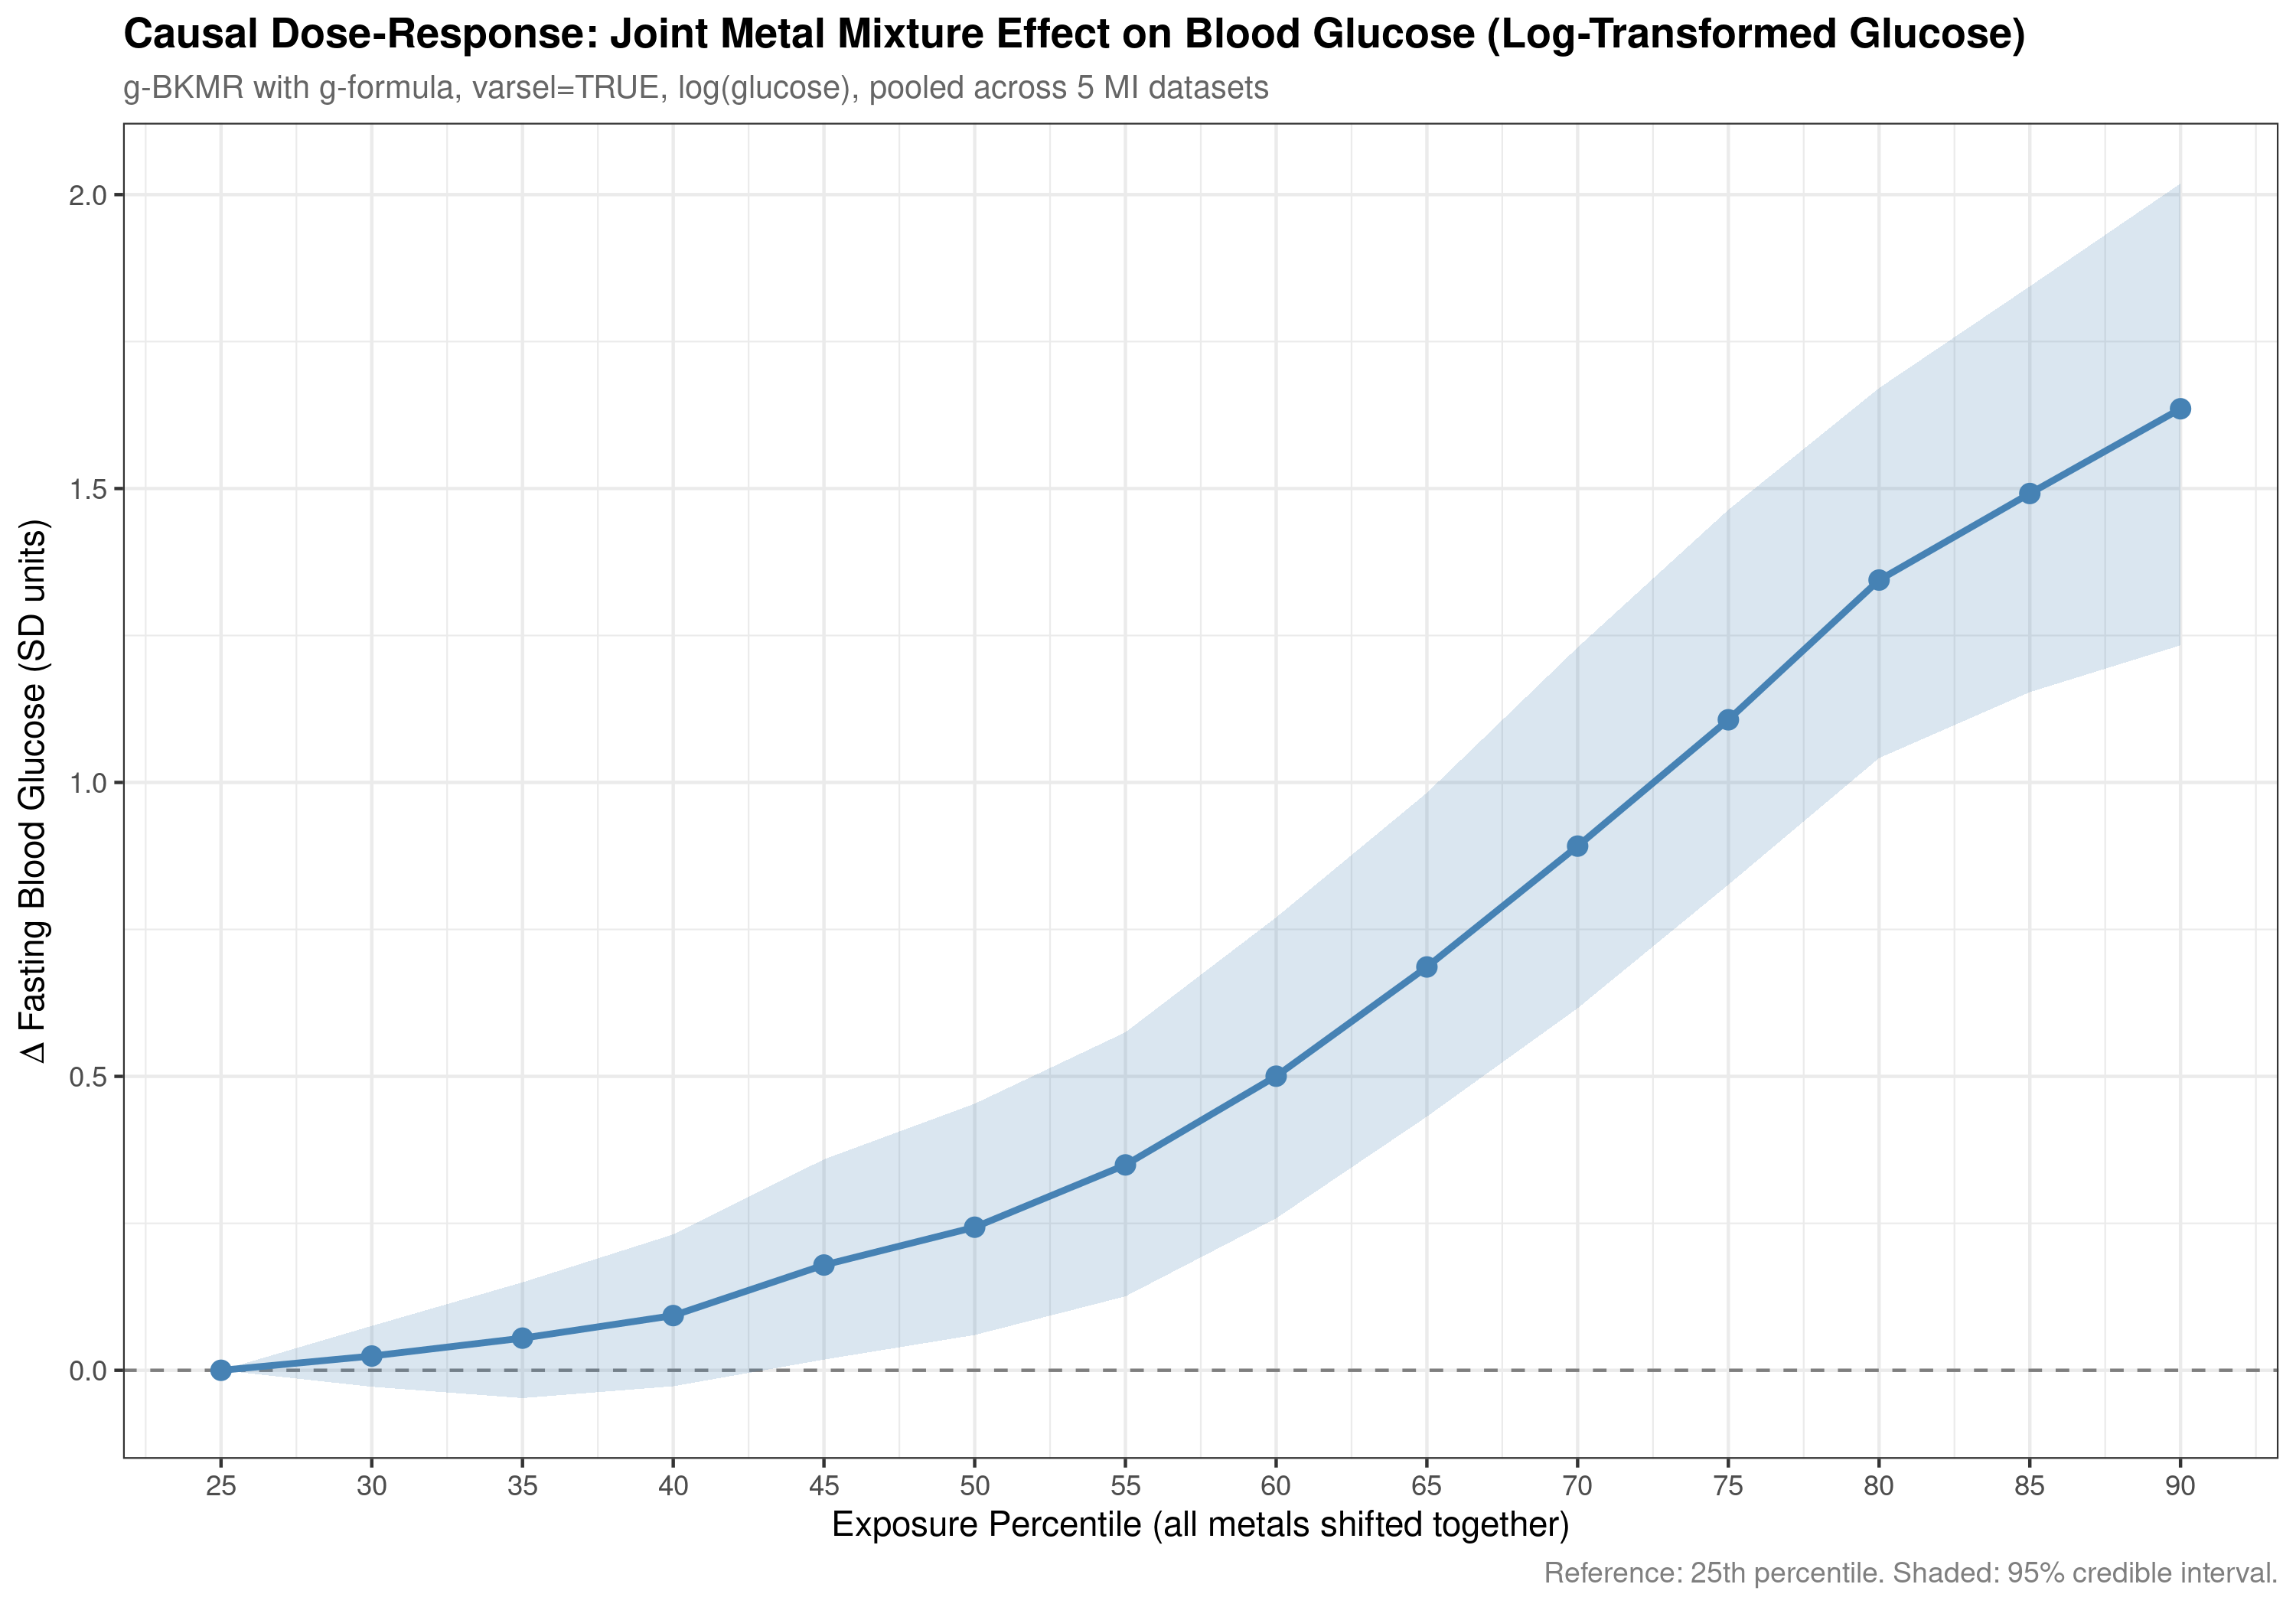
\includegraphics[width=0.85\textwidth]{figures/fig_dr_full.png}
\caption{Joint causal dose-response of the metal mixture on log fasting glucose, full sample ($n = 679$). Reference: 25th percentile. Shaded band: 95\% credible interval.}
\label{fig:dr-joint}
\end{figure}

\begin{figure}[h]
\centering
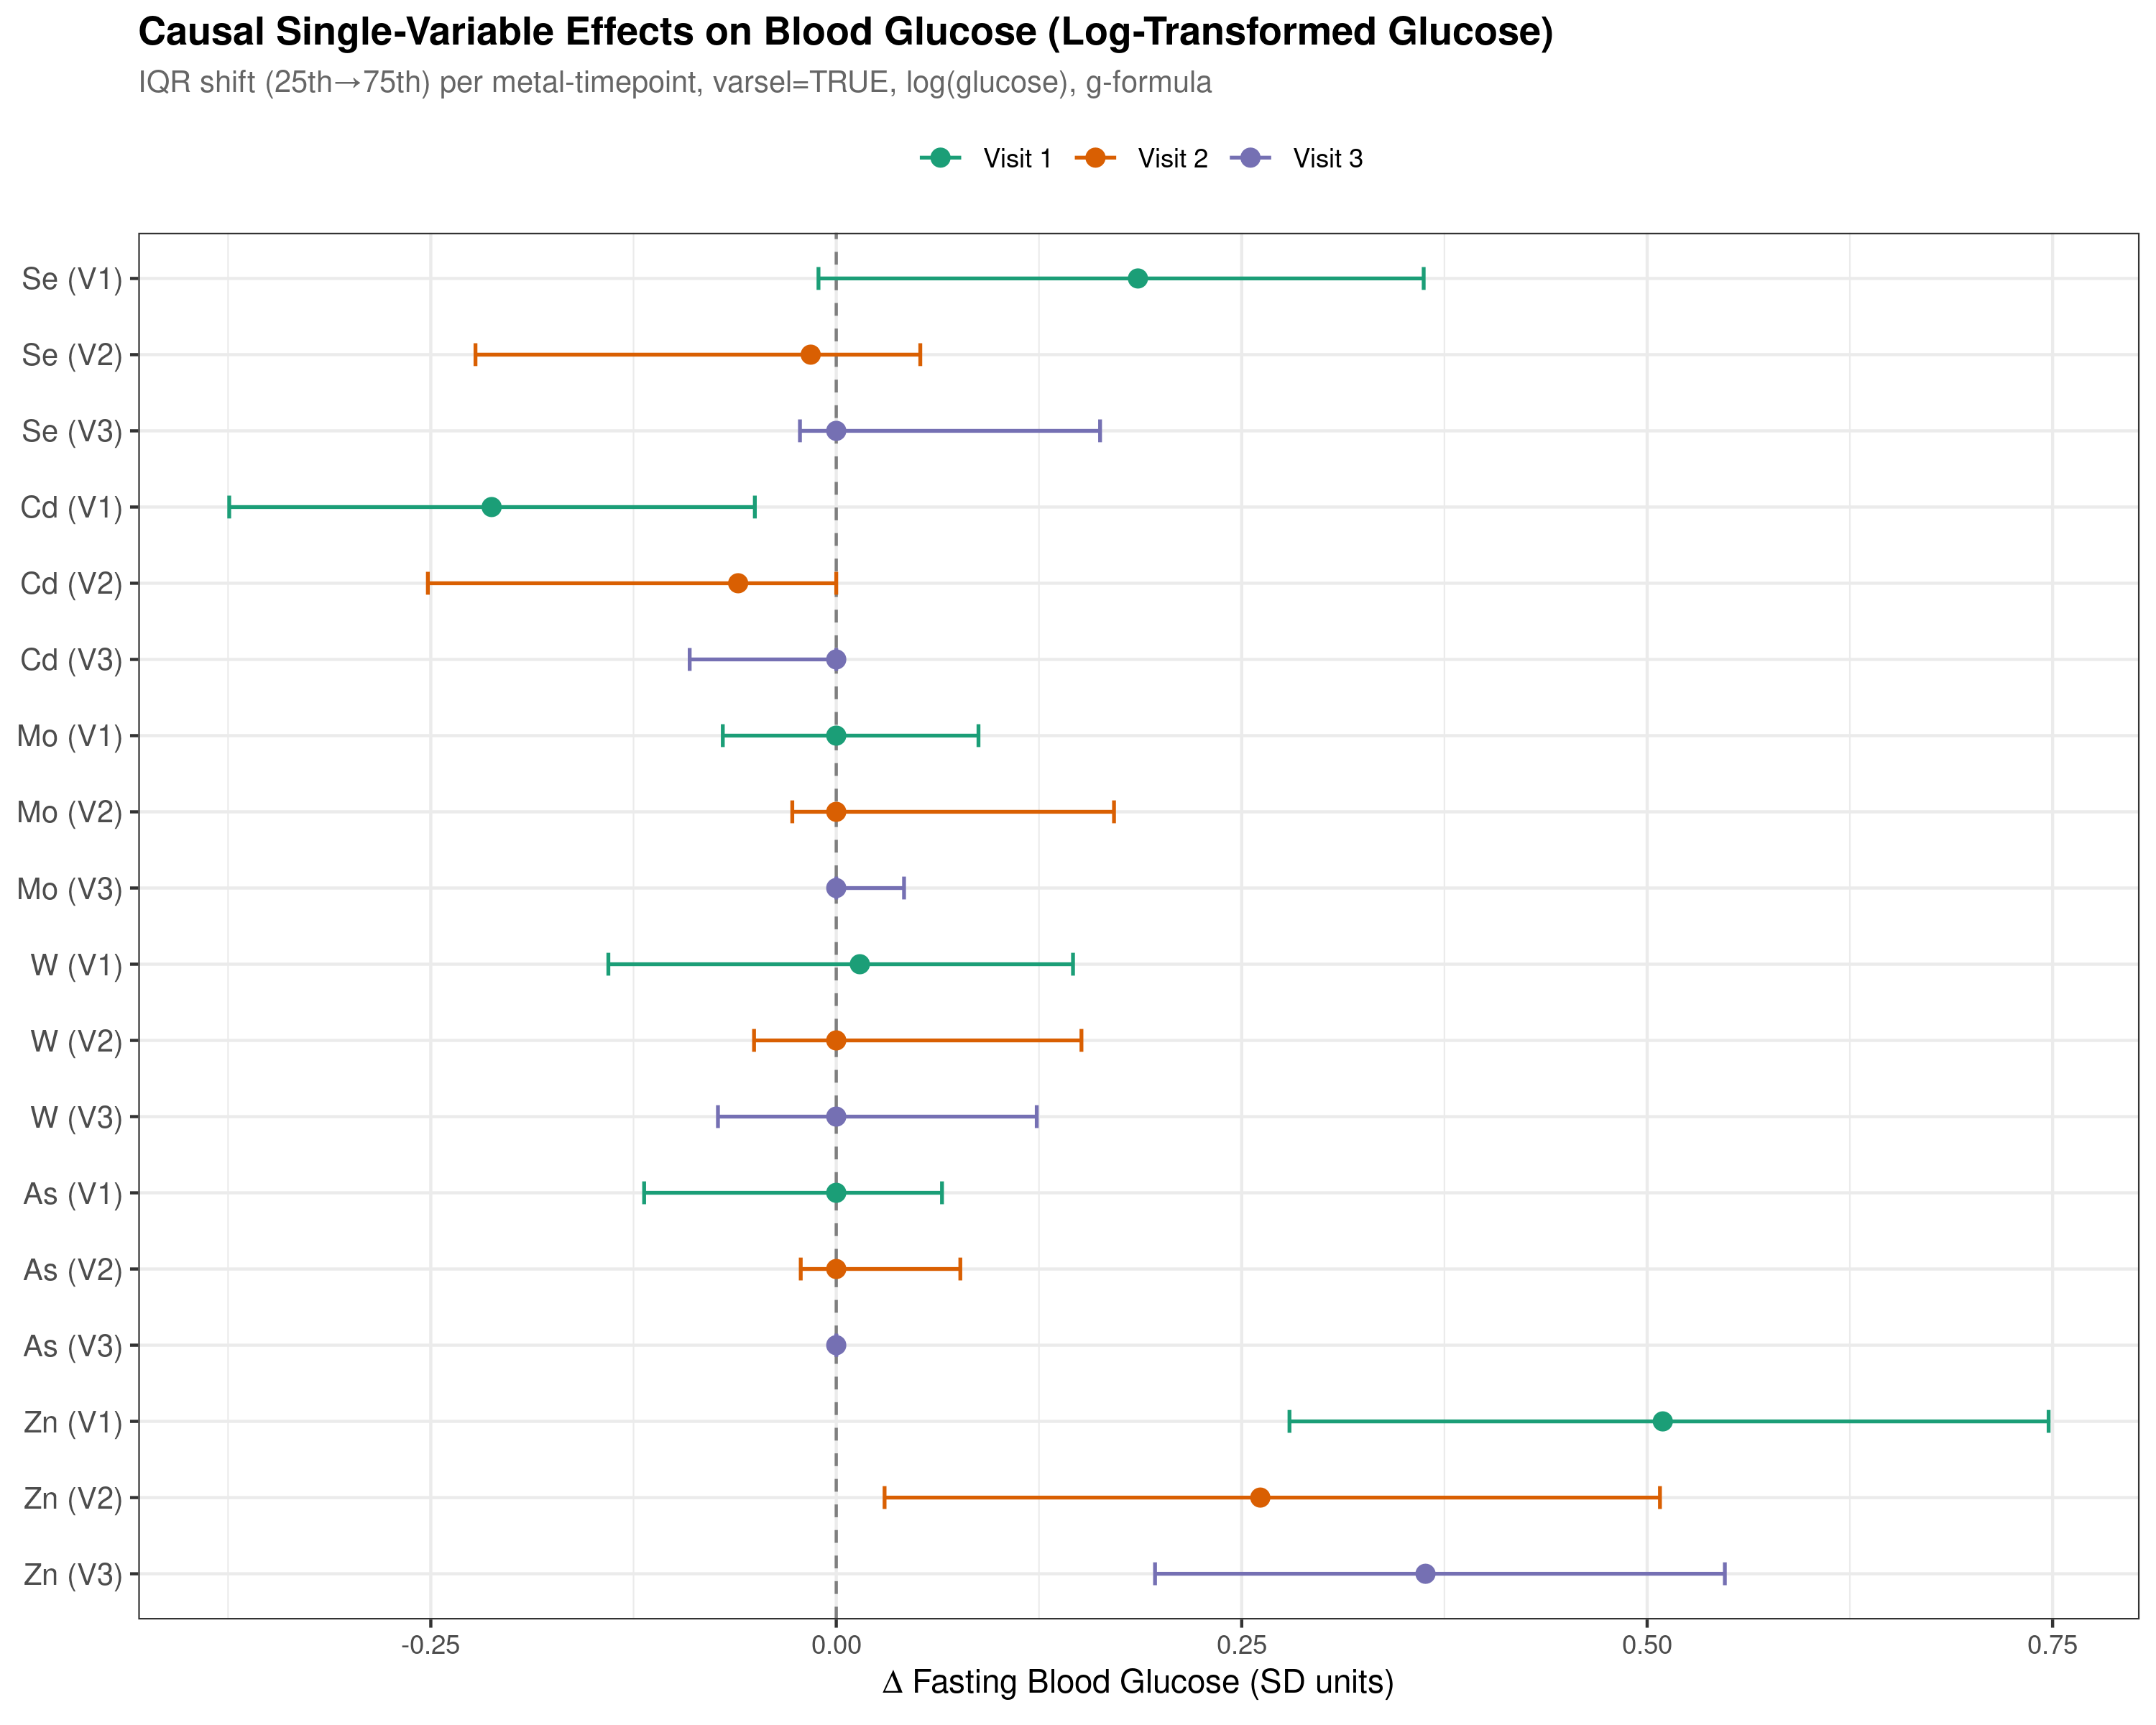
\includegraphics[width=0.85\textwidth]{figures/fig_forest_full.png}
\caption{Single-variable causal effects (IQR shift, 25th to 75th percentile). Bars: 95\% credible intervals. Full sample, $n = 679$.}
\label{fig:forest}
\end{figure}

\begin{figure}[h]
\centering
\begin{subfigure}{0.48\textwidth}
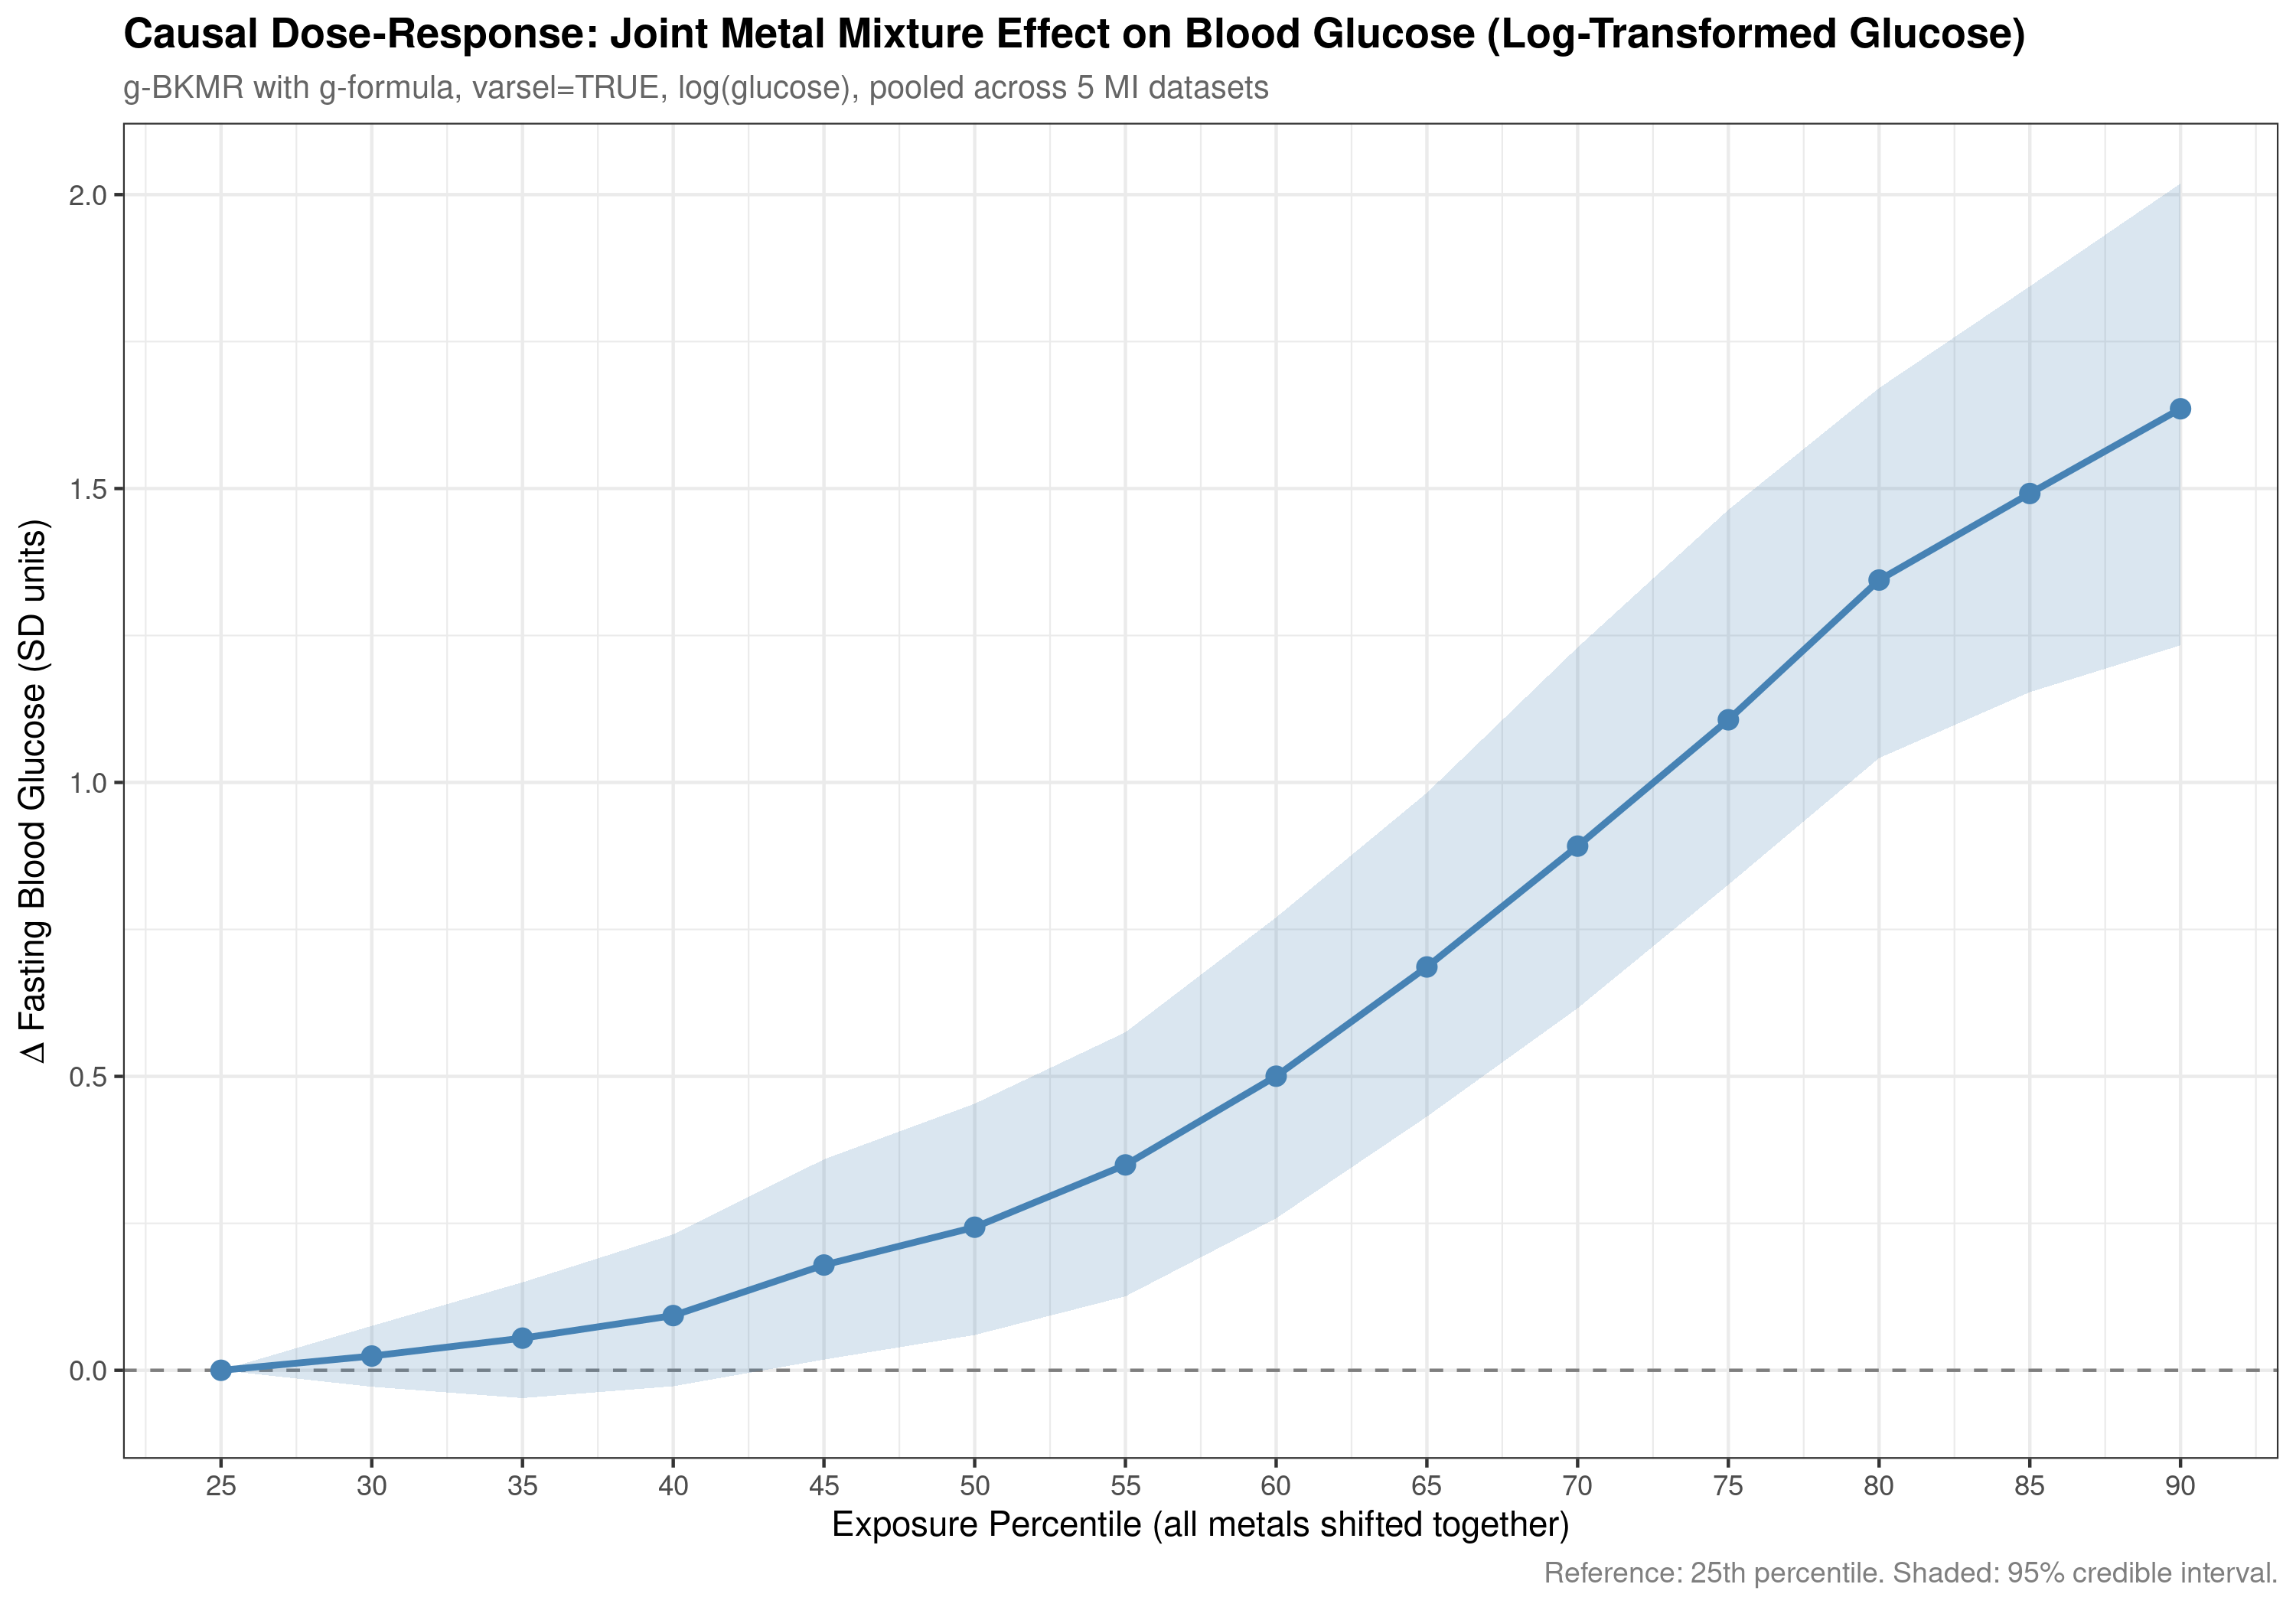
\includegraphics[width=\textwidth]{figures/fig_dr_full.png}
\caption{Full sample ($n = 679$)}
\end{subfigure}\hfill
\begin{subfigure}{0.48\textwidth}
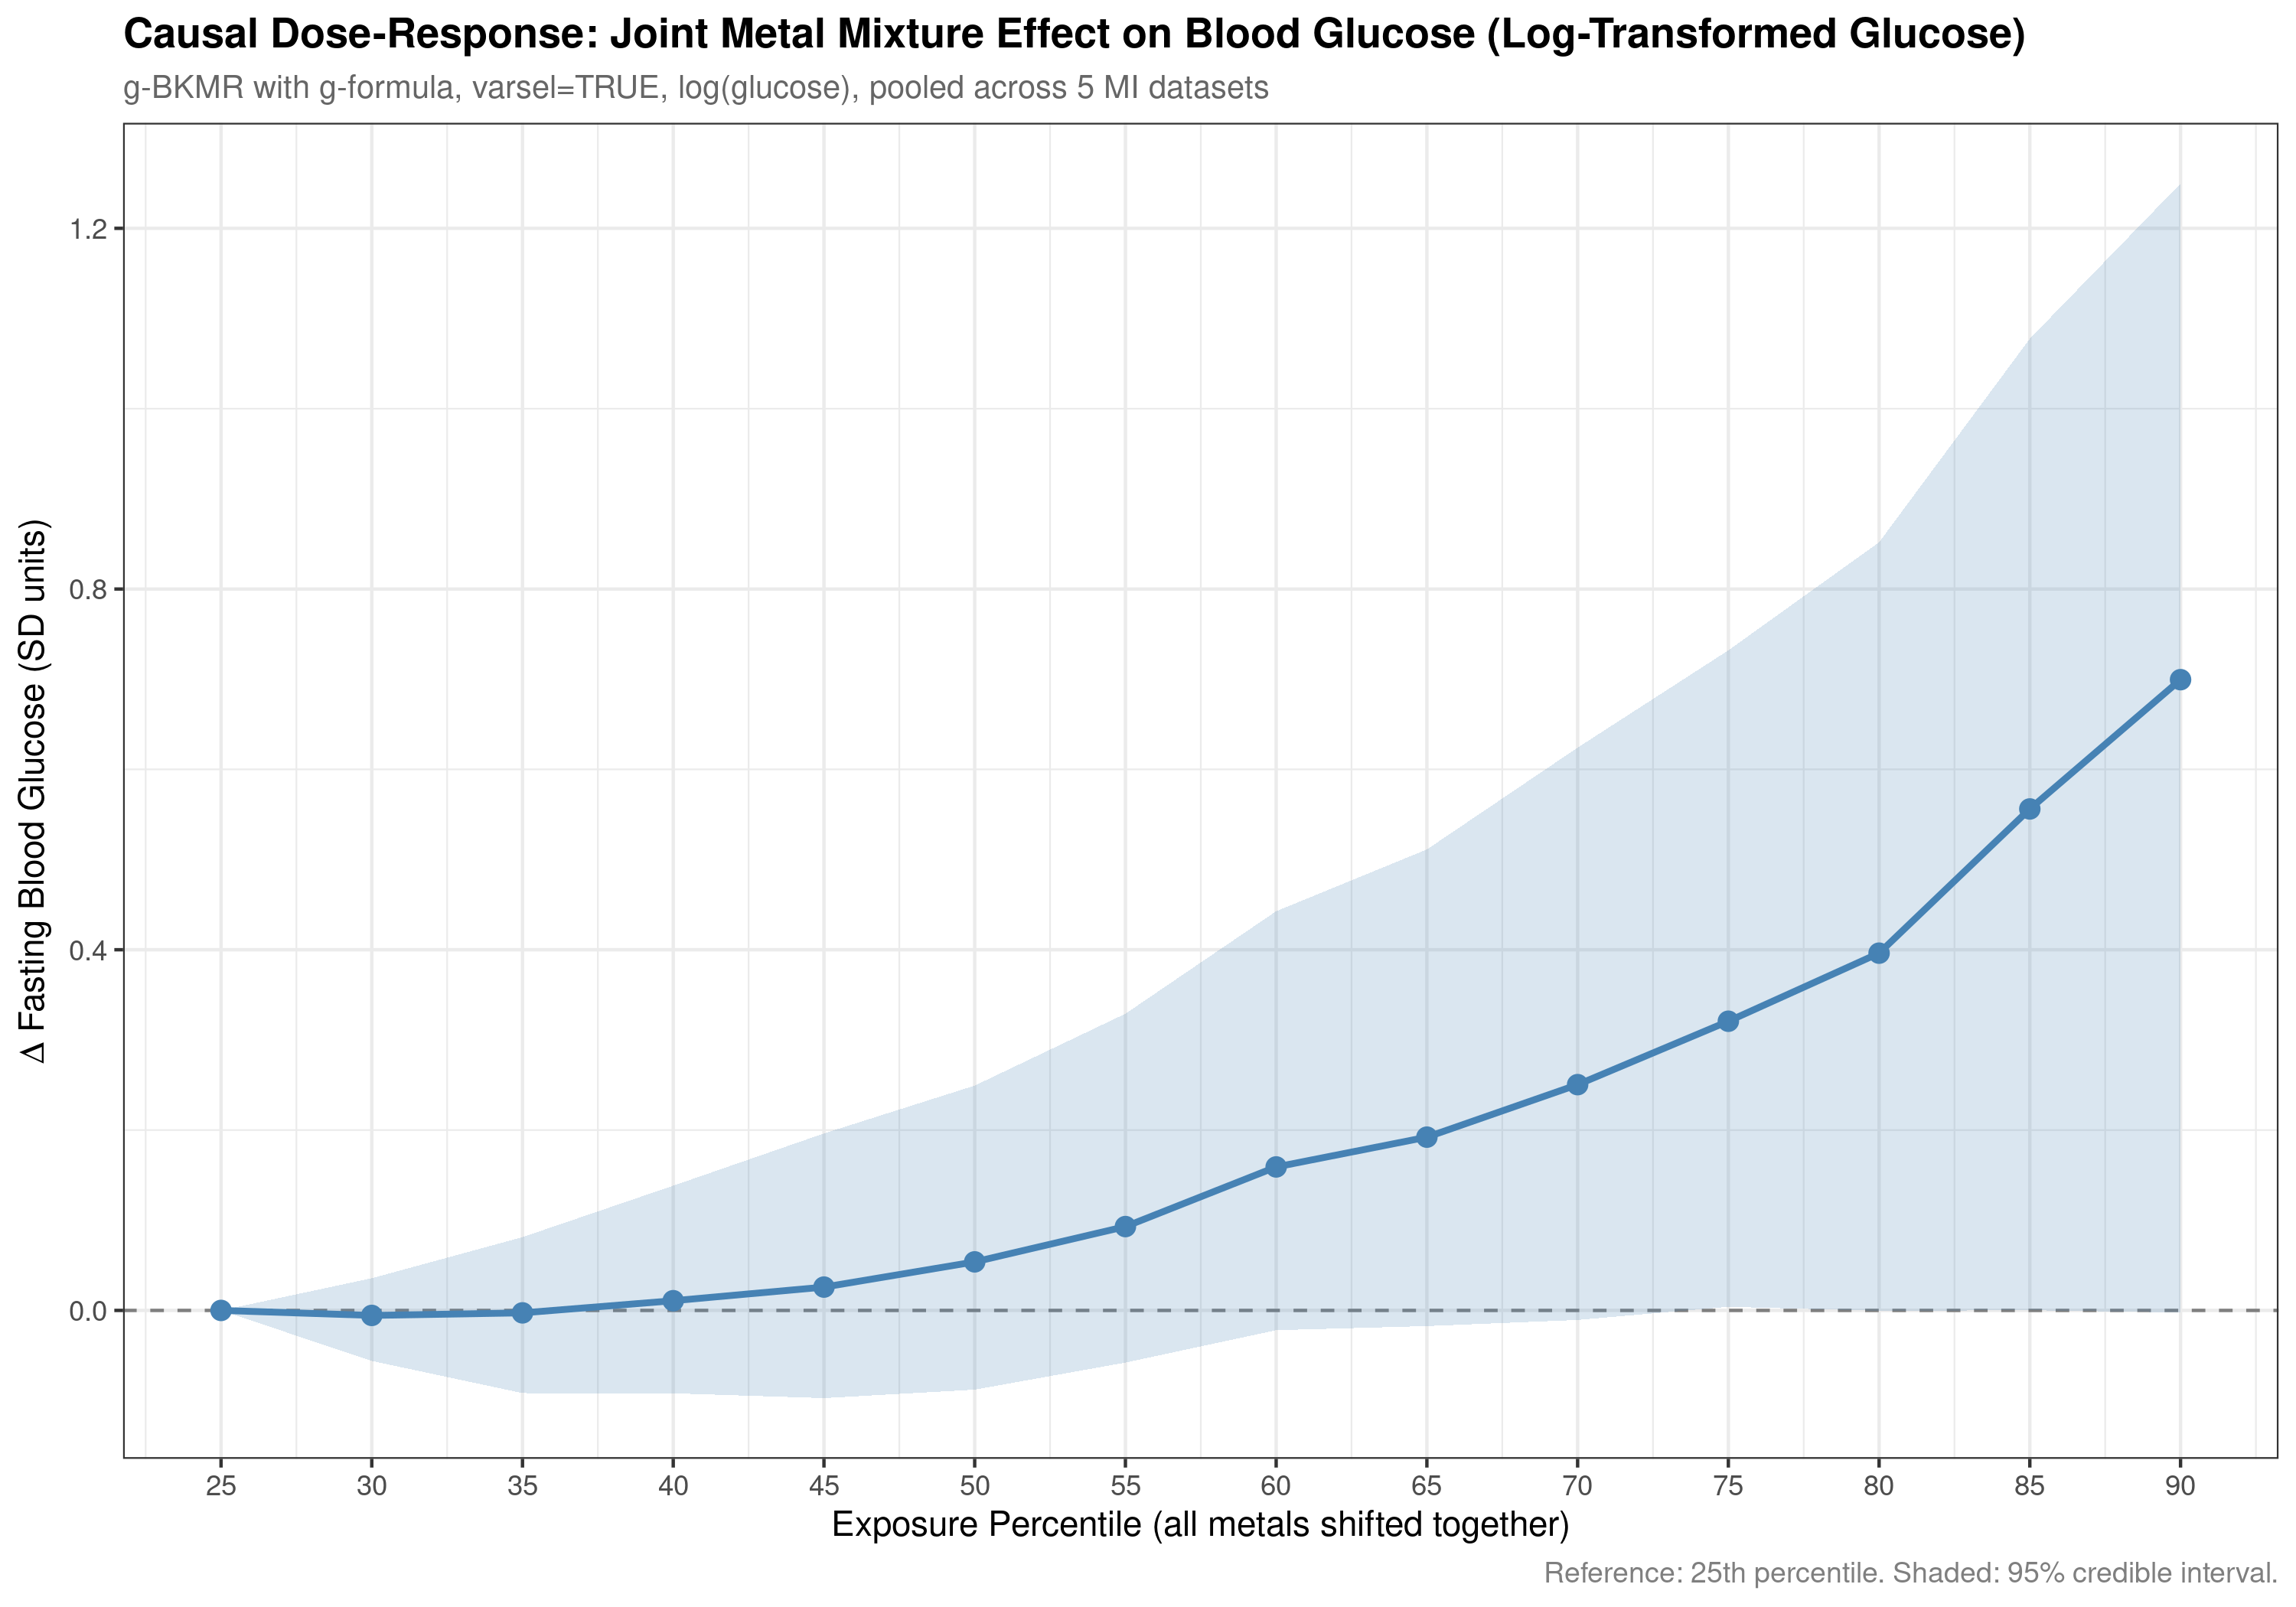
\includegraphics[width=\textwidth]{figures/fig_dr_nodm.png}
\caption{Excluding baseline diabetes ($n = 414$)}
\end{subfigure}
\caption{Sensitivity: joint dose-response in full sample (left) vs.\ excluding baseline diabetes (right).}
\label{fig:dr-compare}
\end{figure}

% ============================================================================
% SUPPLEMENTARY FIGURES
% ============================================================================
\clearpage
\section*{Supplementary Material}

\begin{figure}[h]
\centering
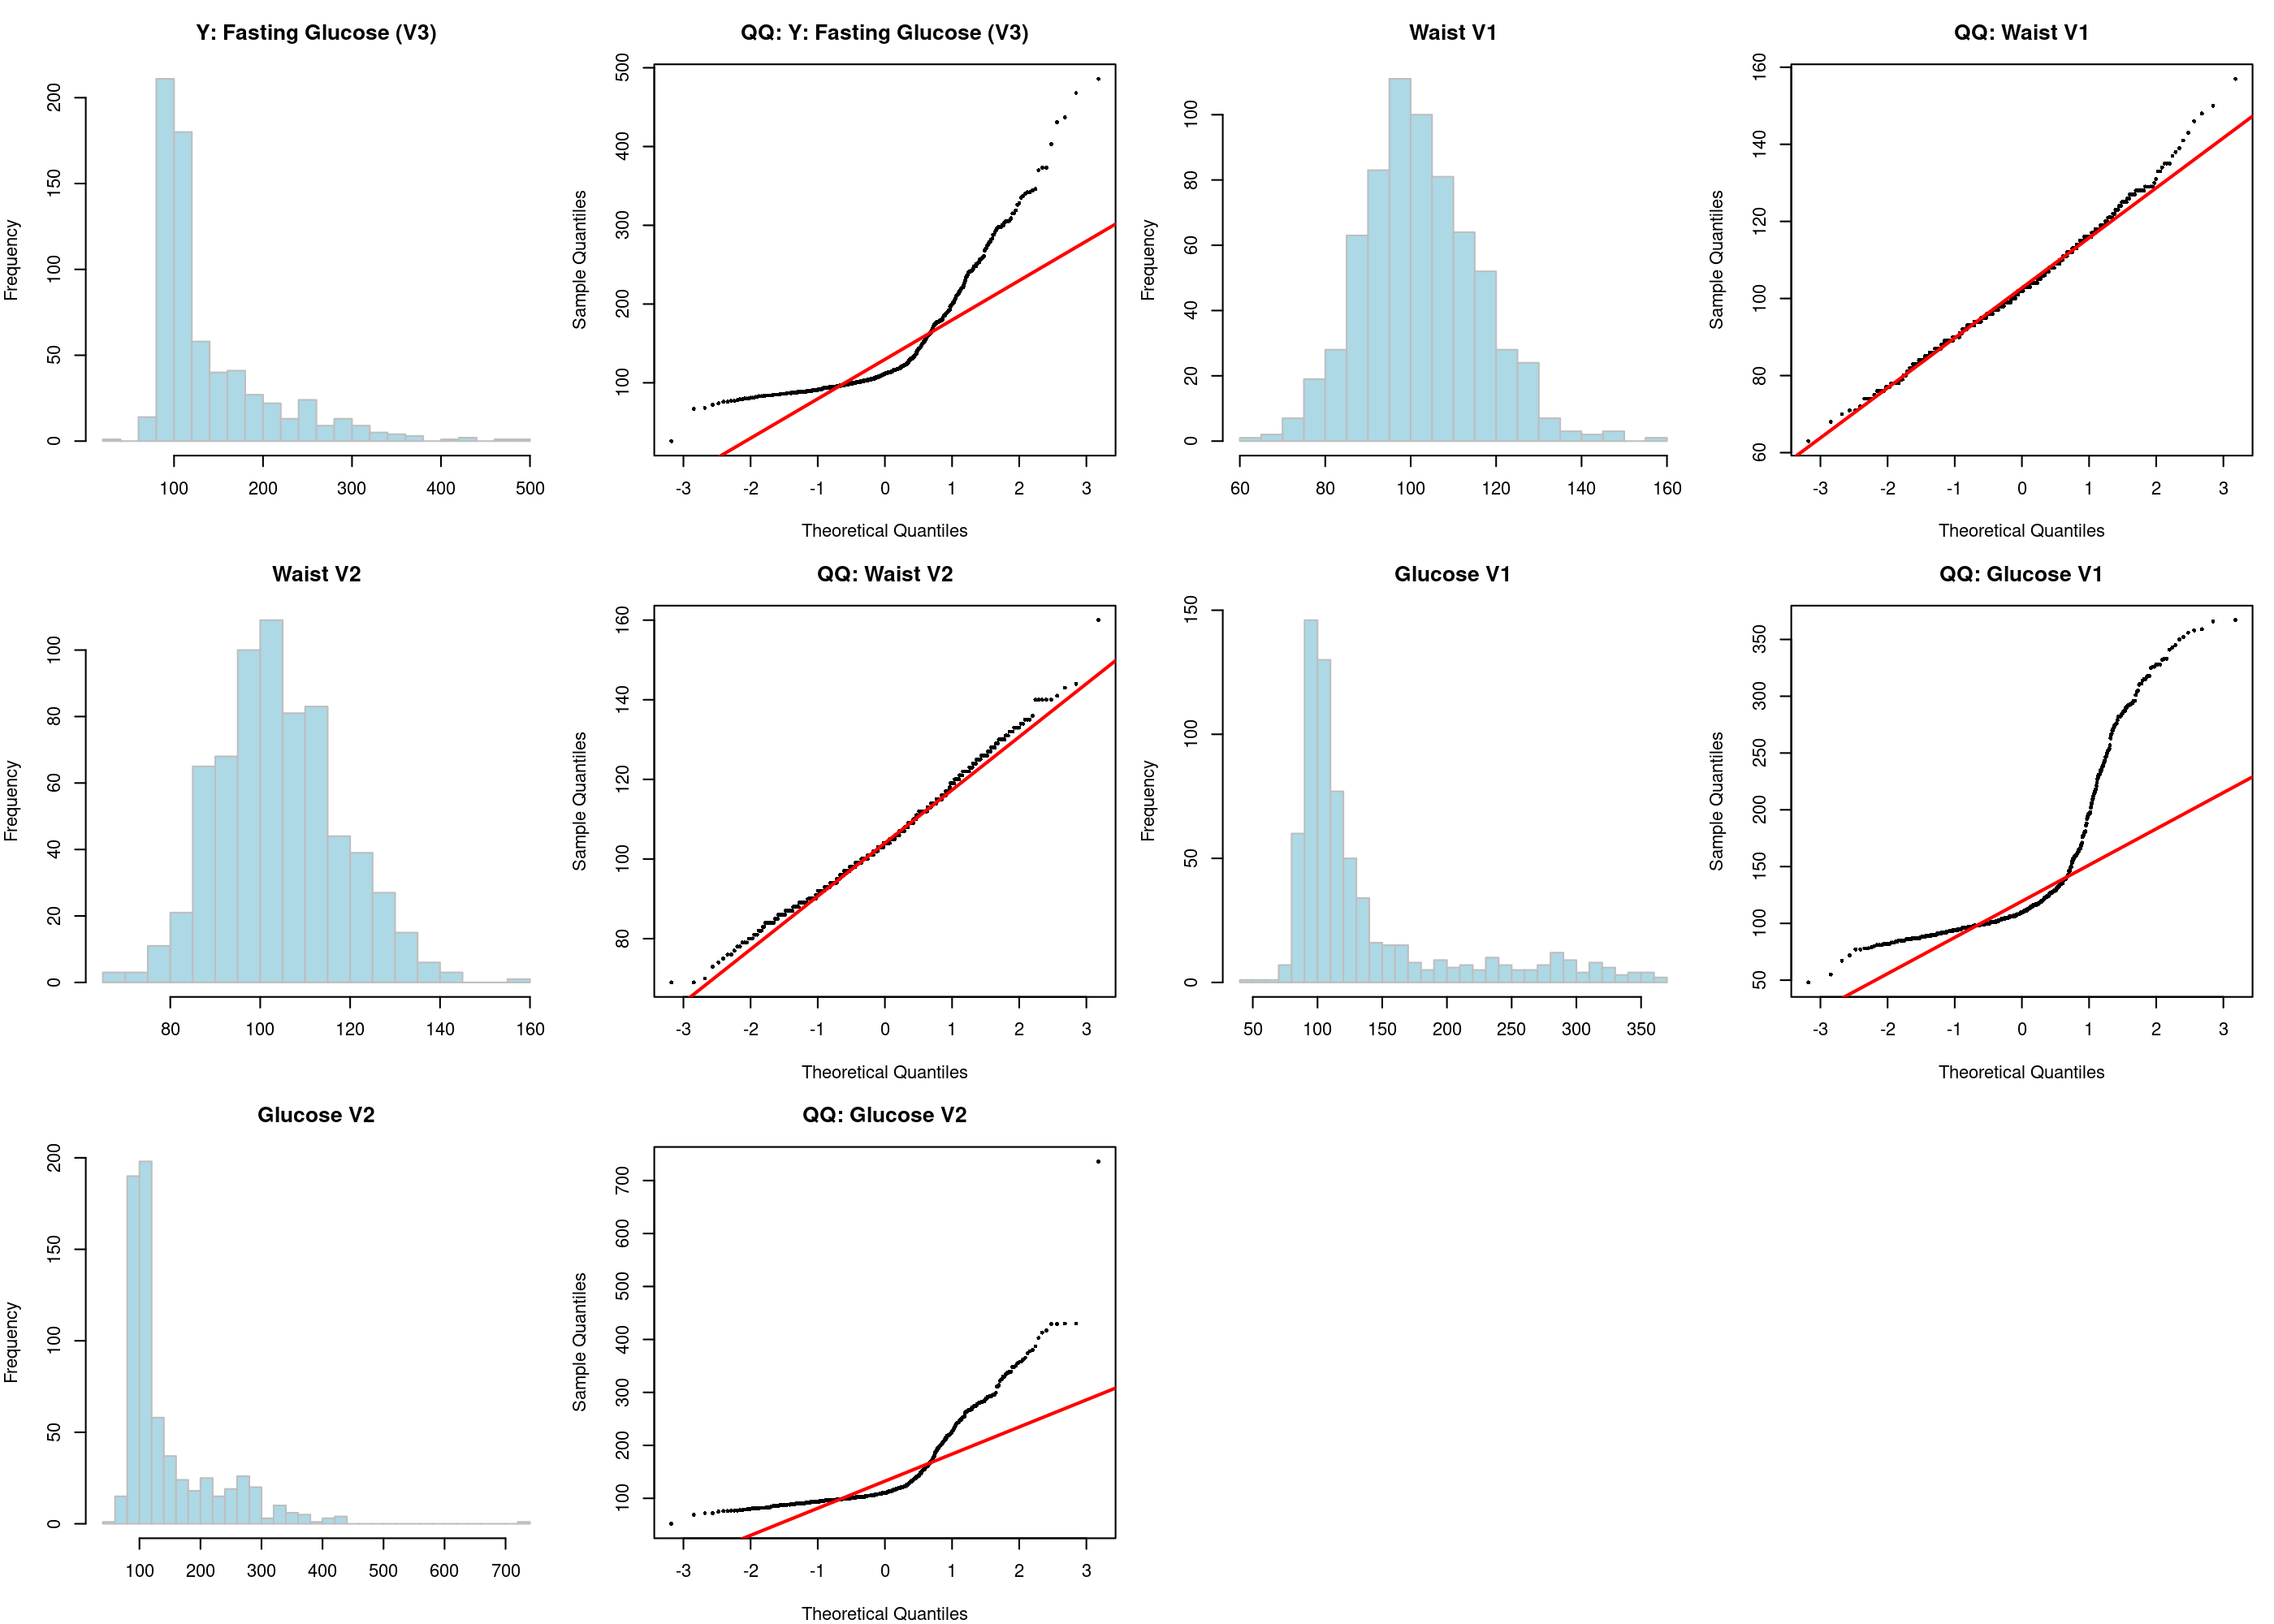
\includegraphics[width=0.85\textwidth]{figures/fig_diagnostic_distributions.png}
\caption{Distribution of outcome and time-varying covariates. Fasting glucose variables are right-skewed (skewness $1.8$--$2.1$), motivating log transformation.}
\label{fig:supp-dist}
\end{figure}

\begin{figure}[h]
\centering
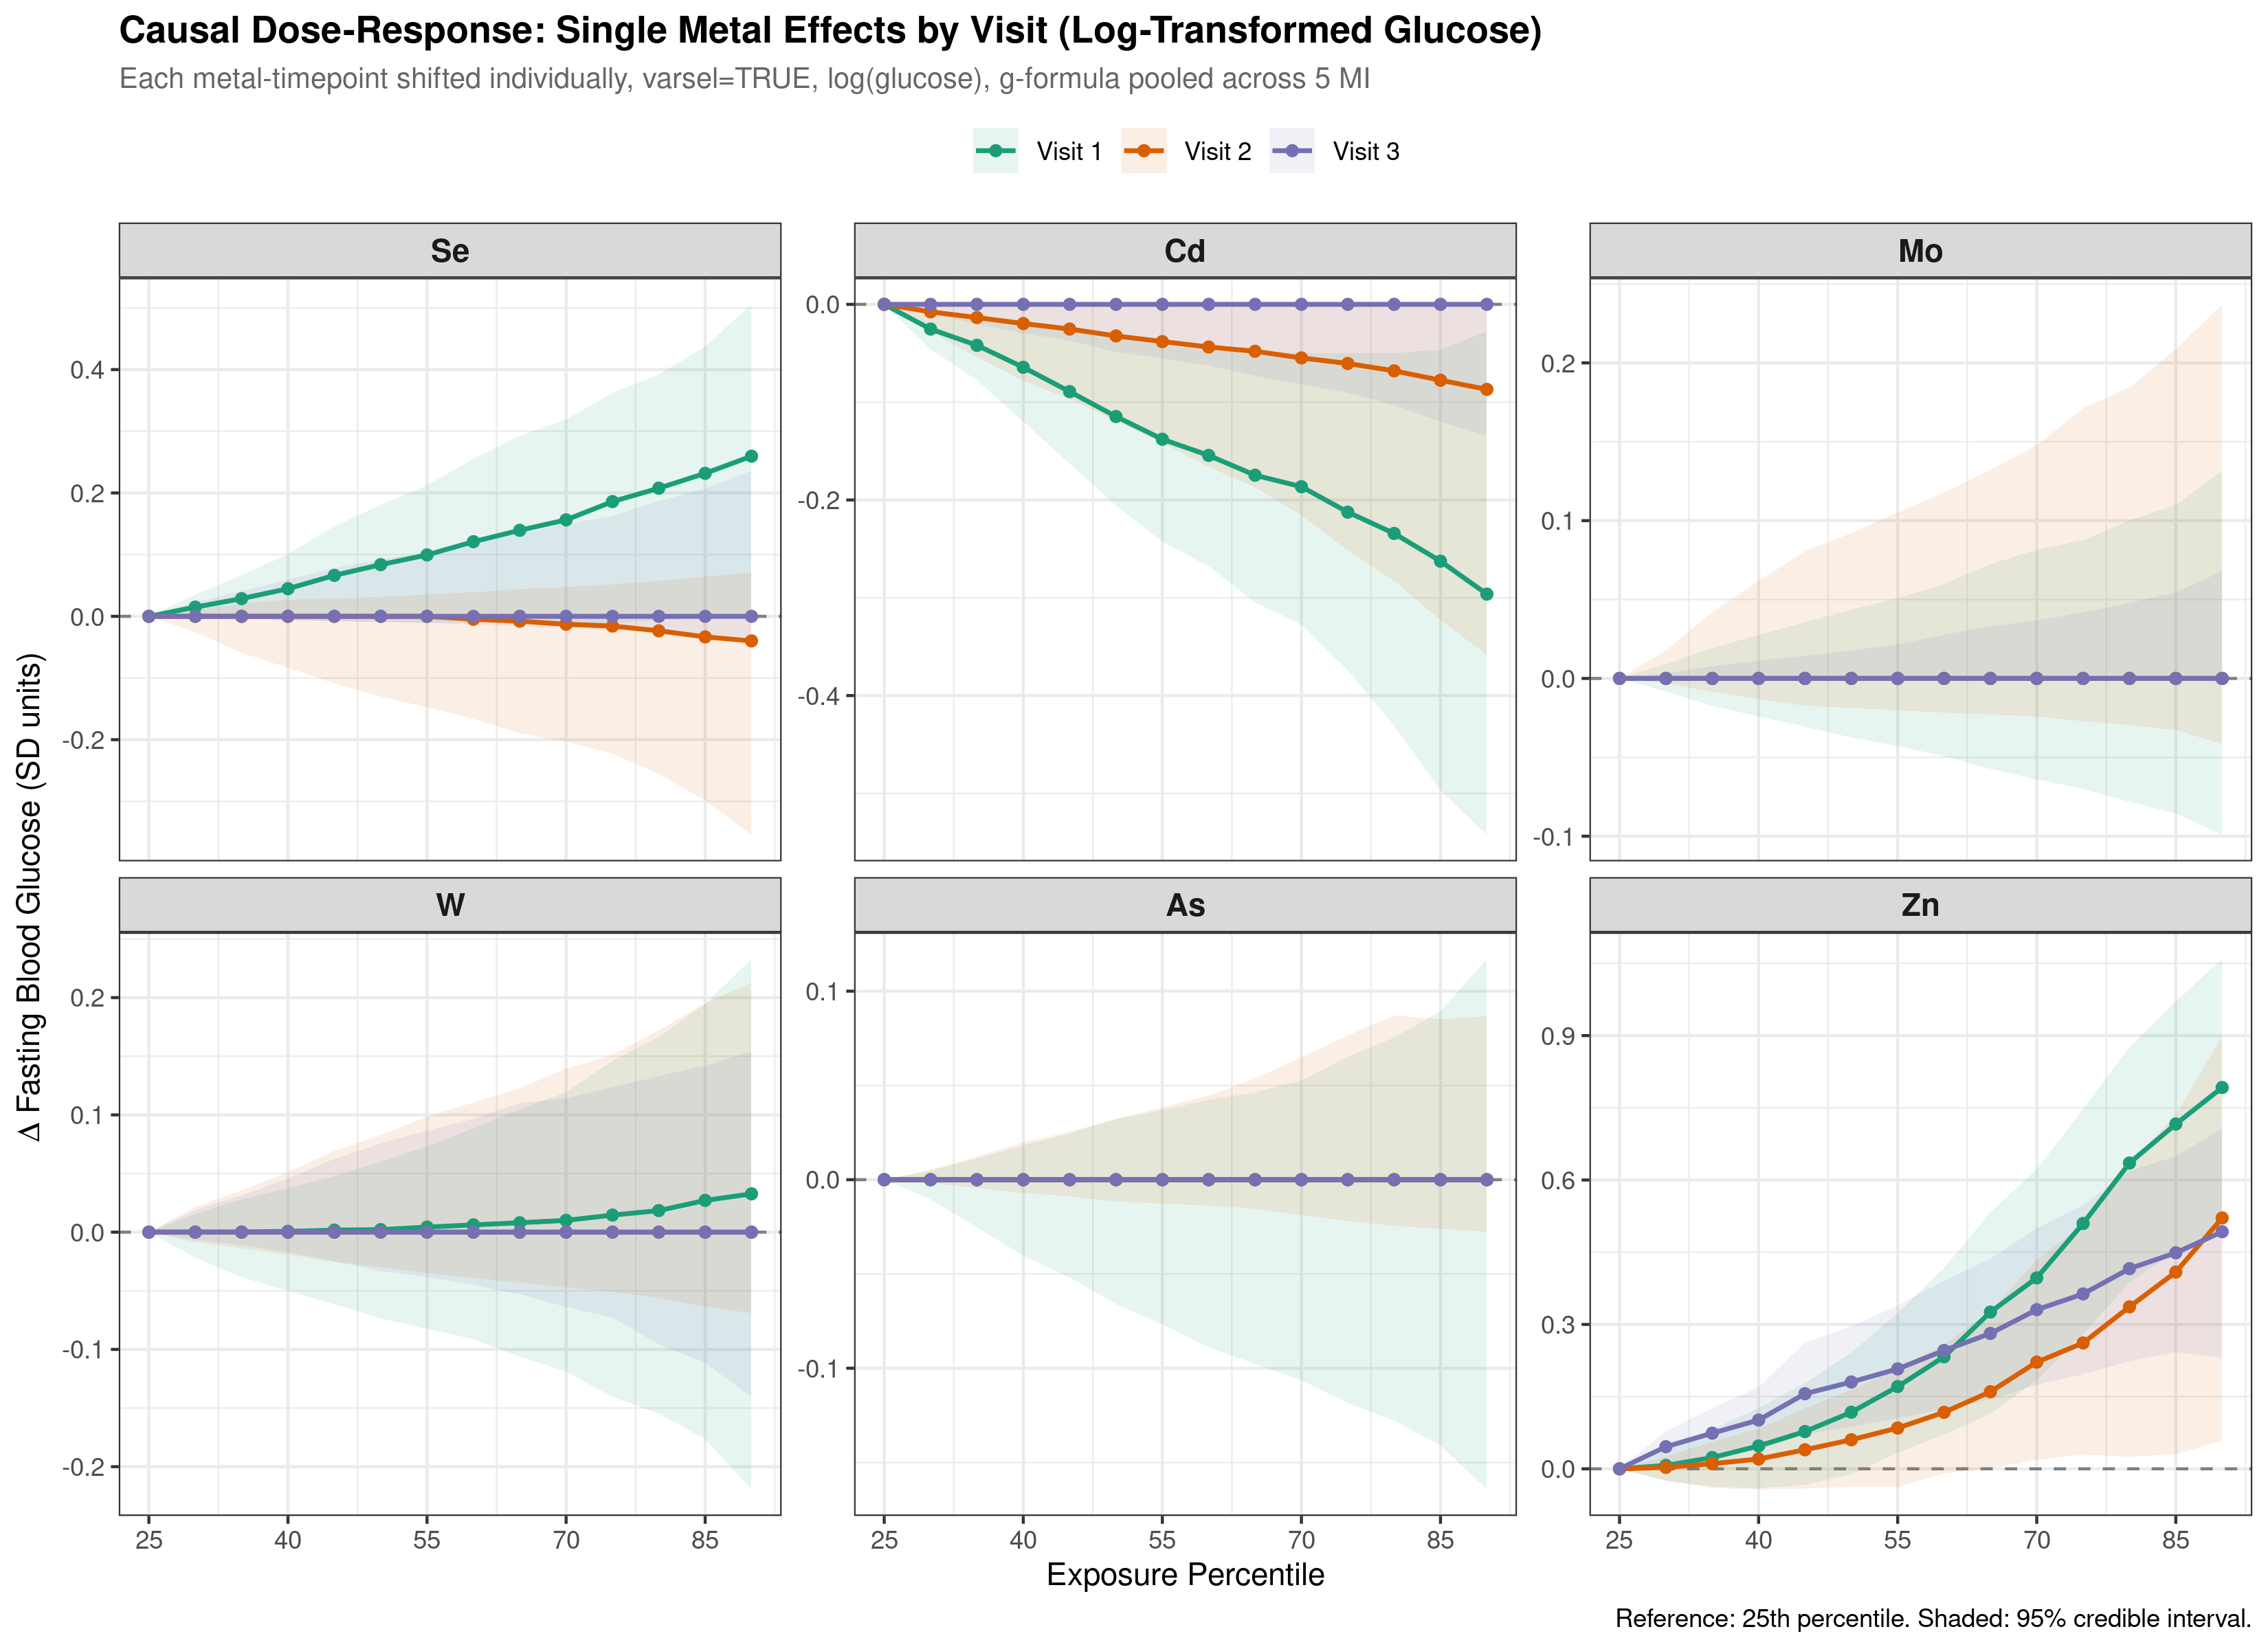
\includegraphics[width=0.85\textwidth]{figures/fig_permetal_full.png}
\caption{Per-metal dose-response curves (full sample). Each panel: one metal shifted across percentiles, remaining exposures at the 50th percentile. Lines distinguish the three visits.}
\label{fig:supp-permetal}
\end{figure}

\begin{figure}[h]
\centering
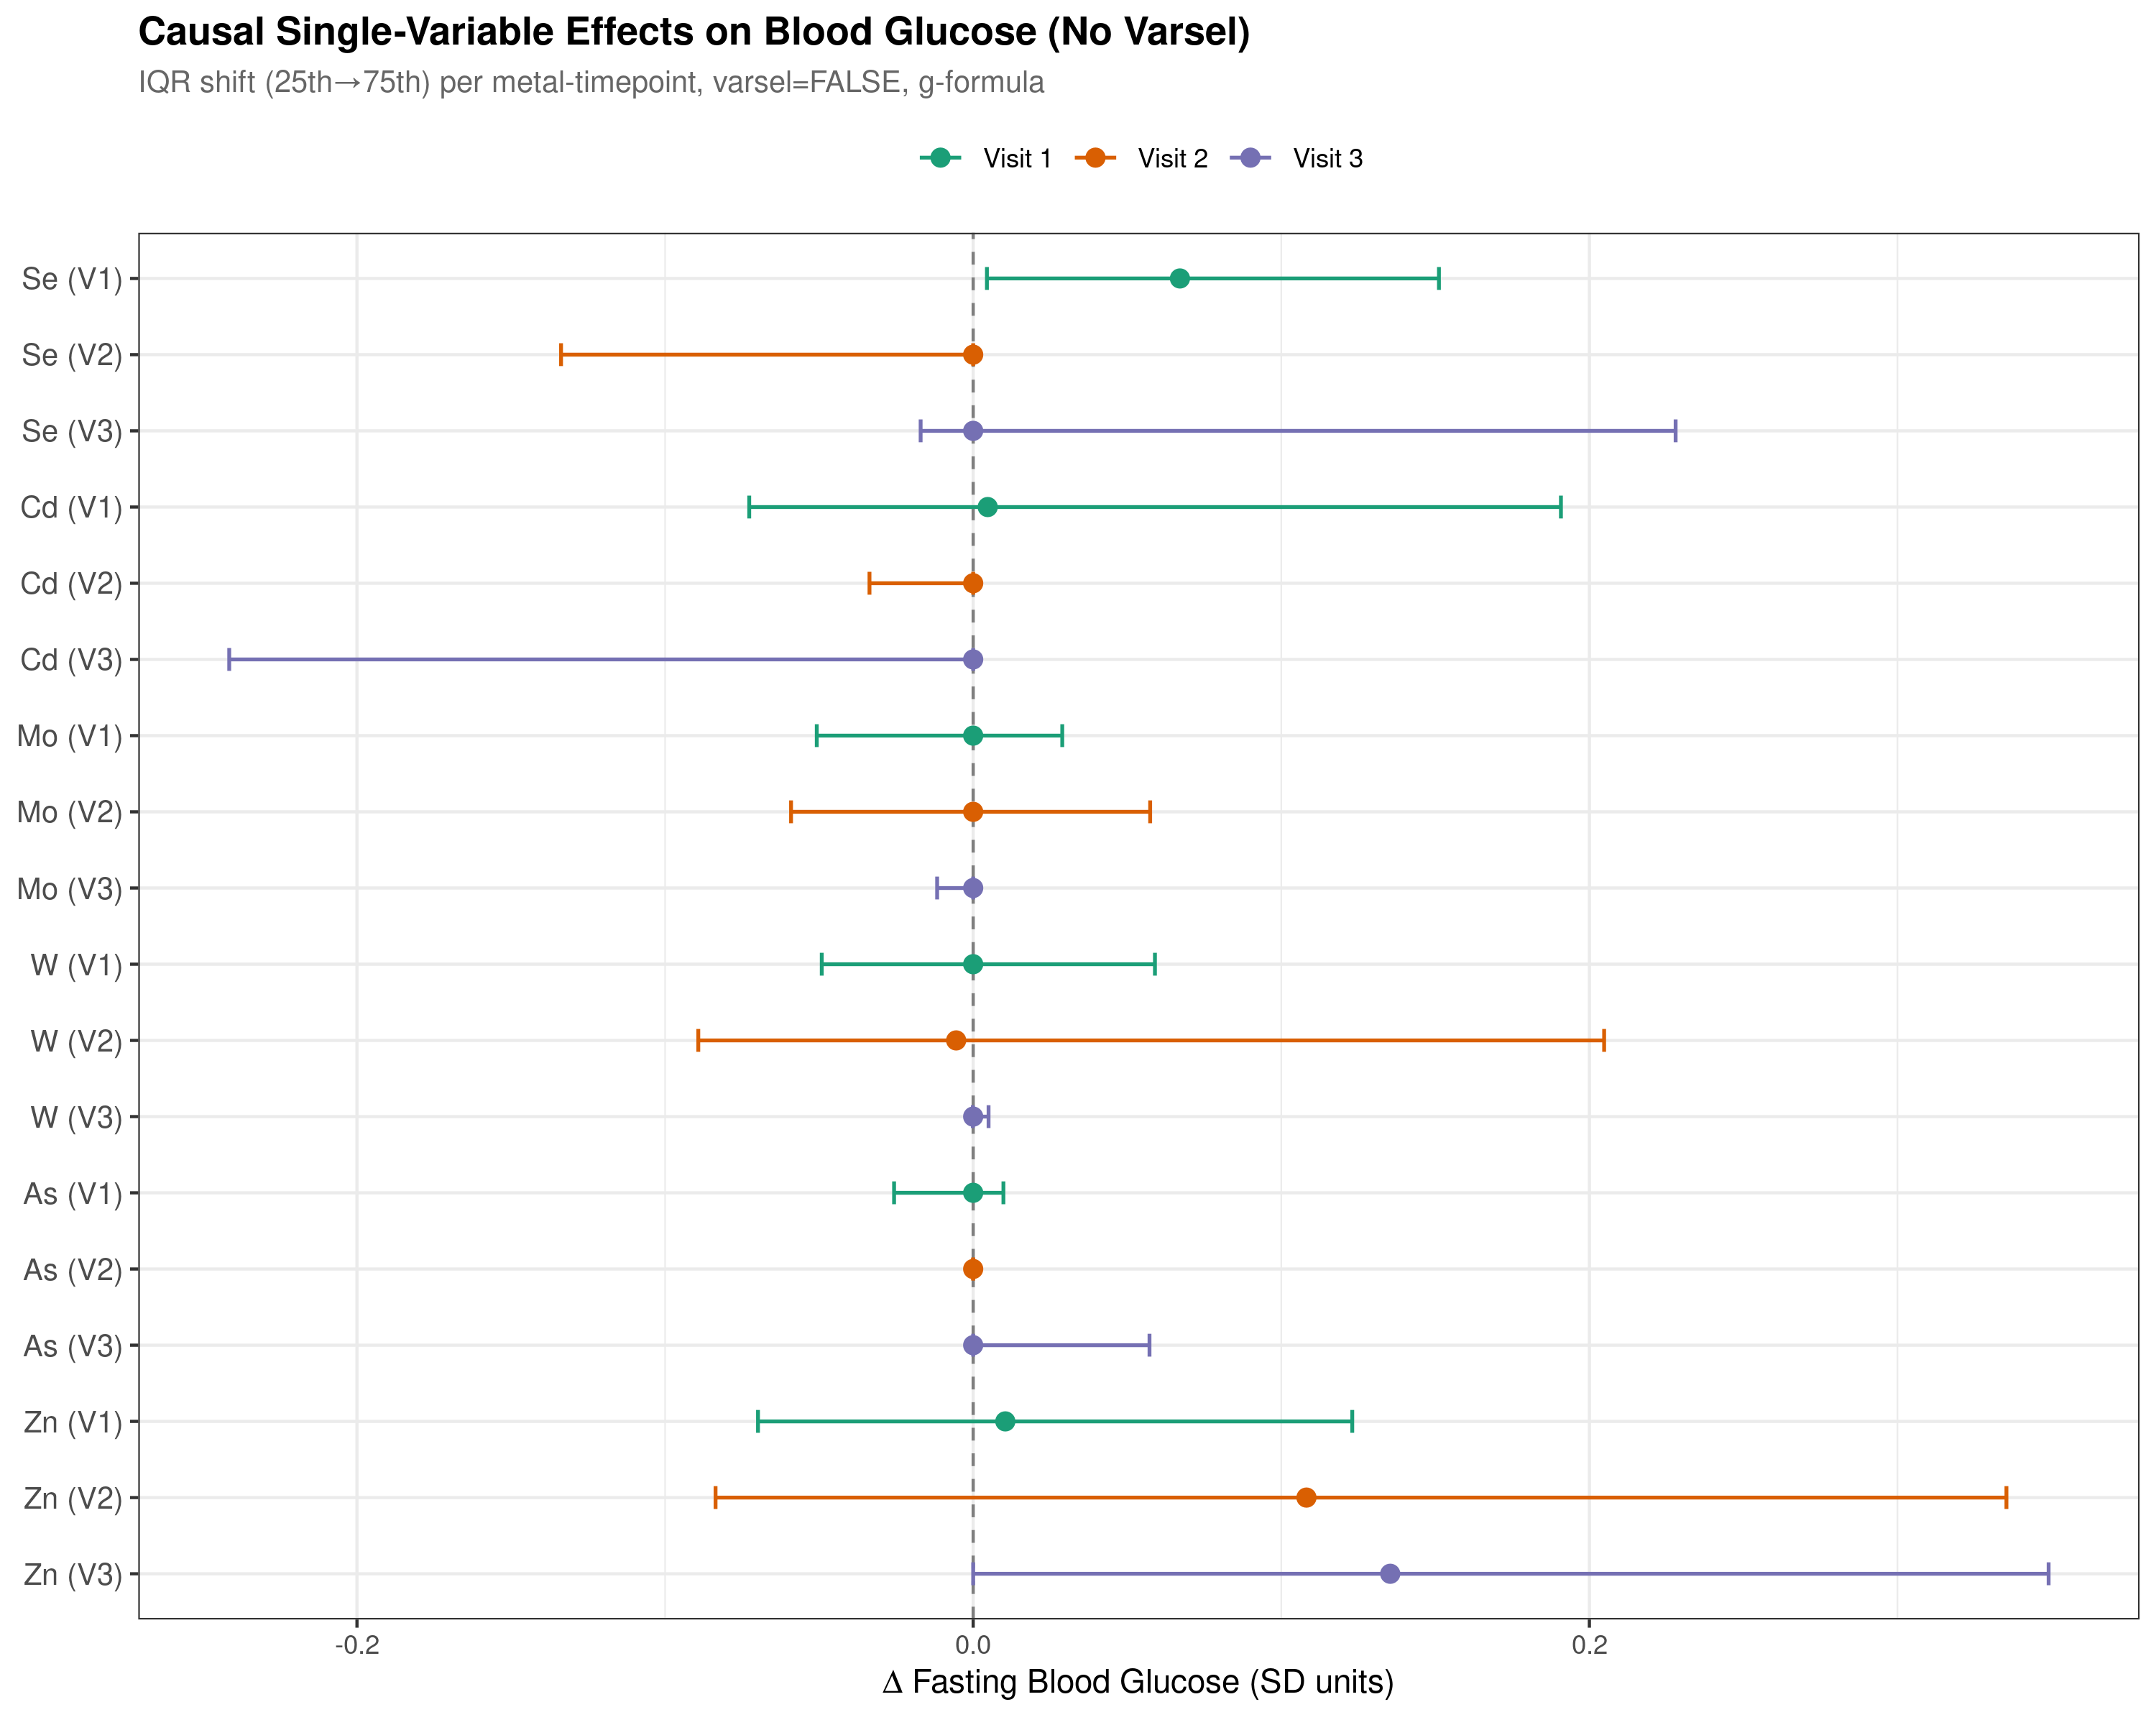
\includegraphics[width=0.85\textwidth]{figures/fig_forest_nodm.png}
\caption{Single-variable causal effects, excluding baseline diabetes ($n = 414$).}
\label{fig:supp-forest-nodm}
\end{figure}

\begin{figure}[h]
\centering
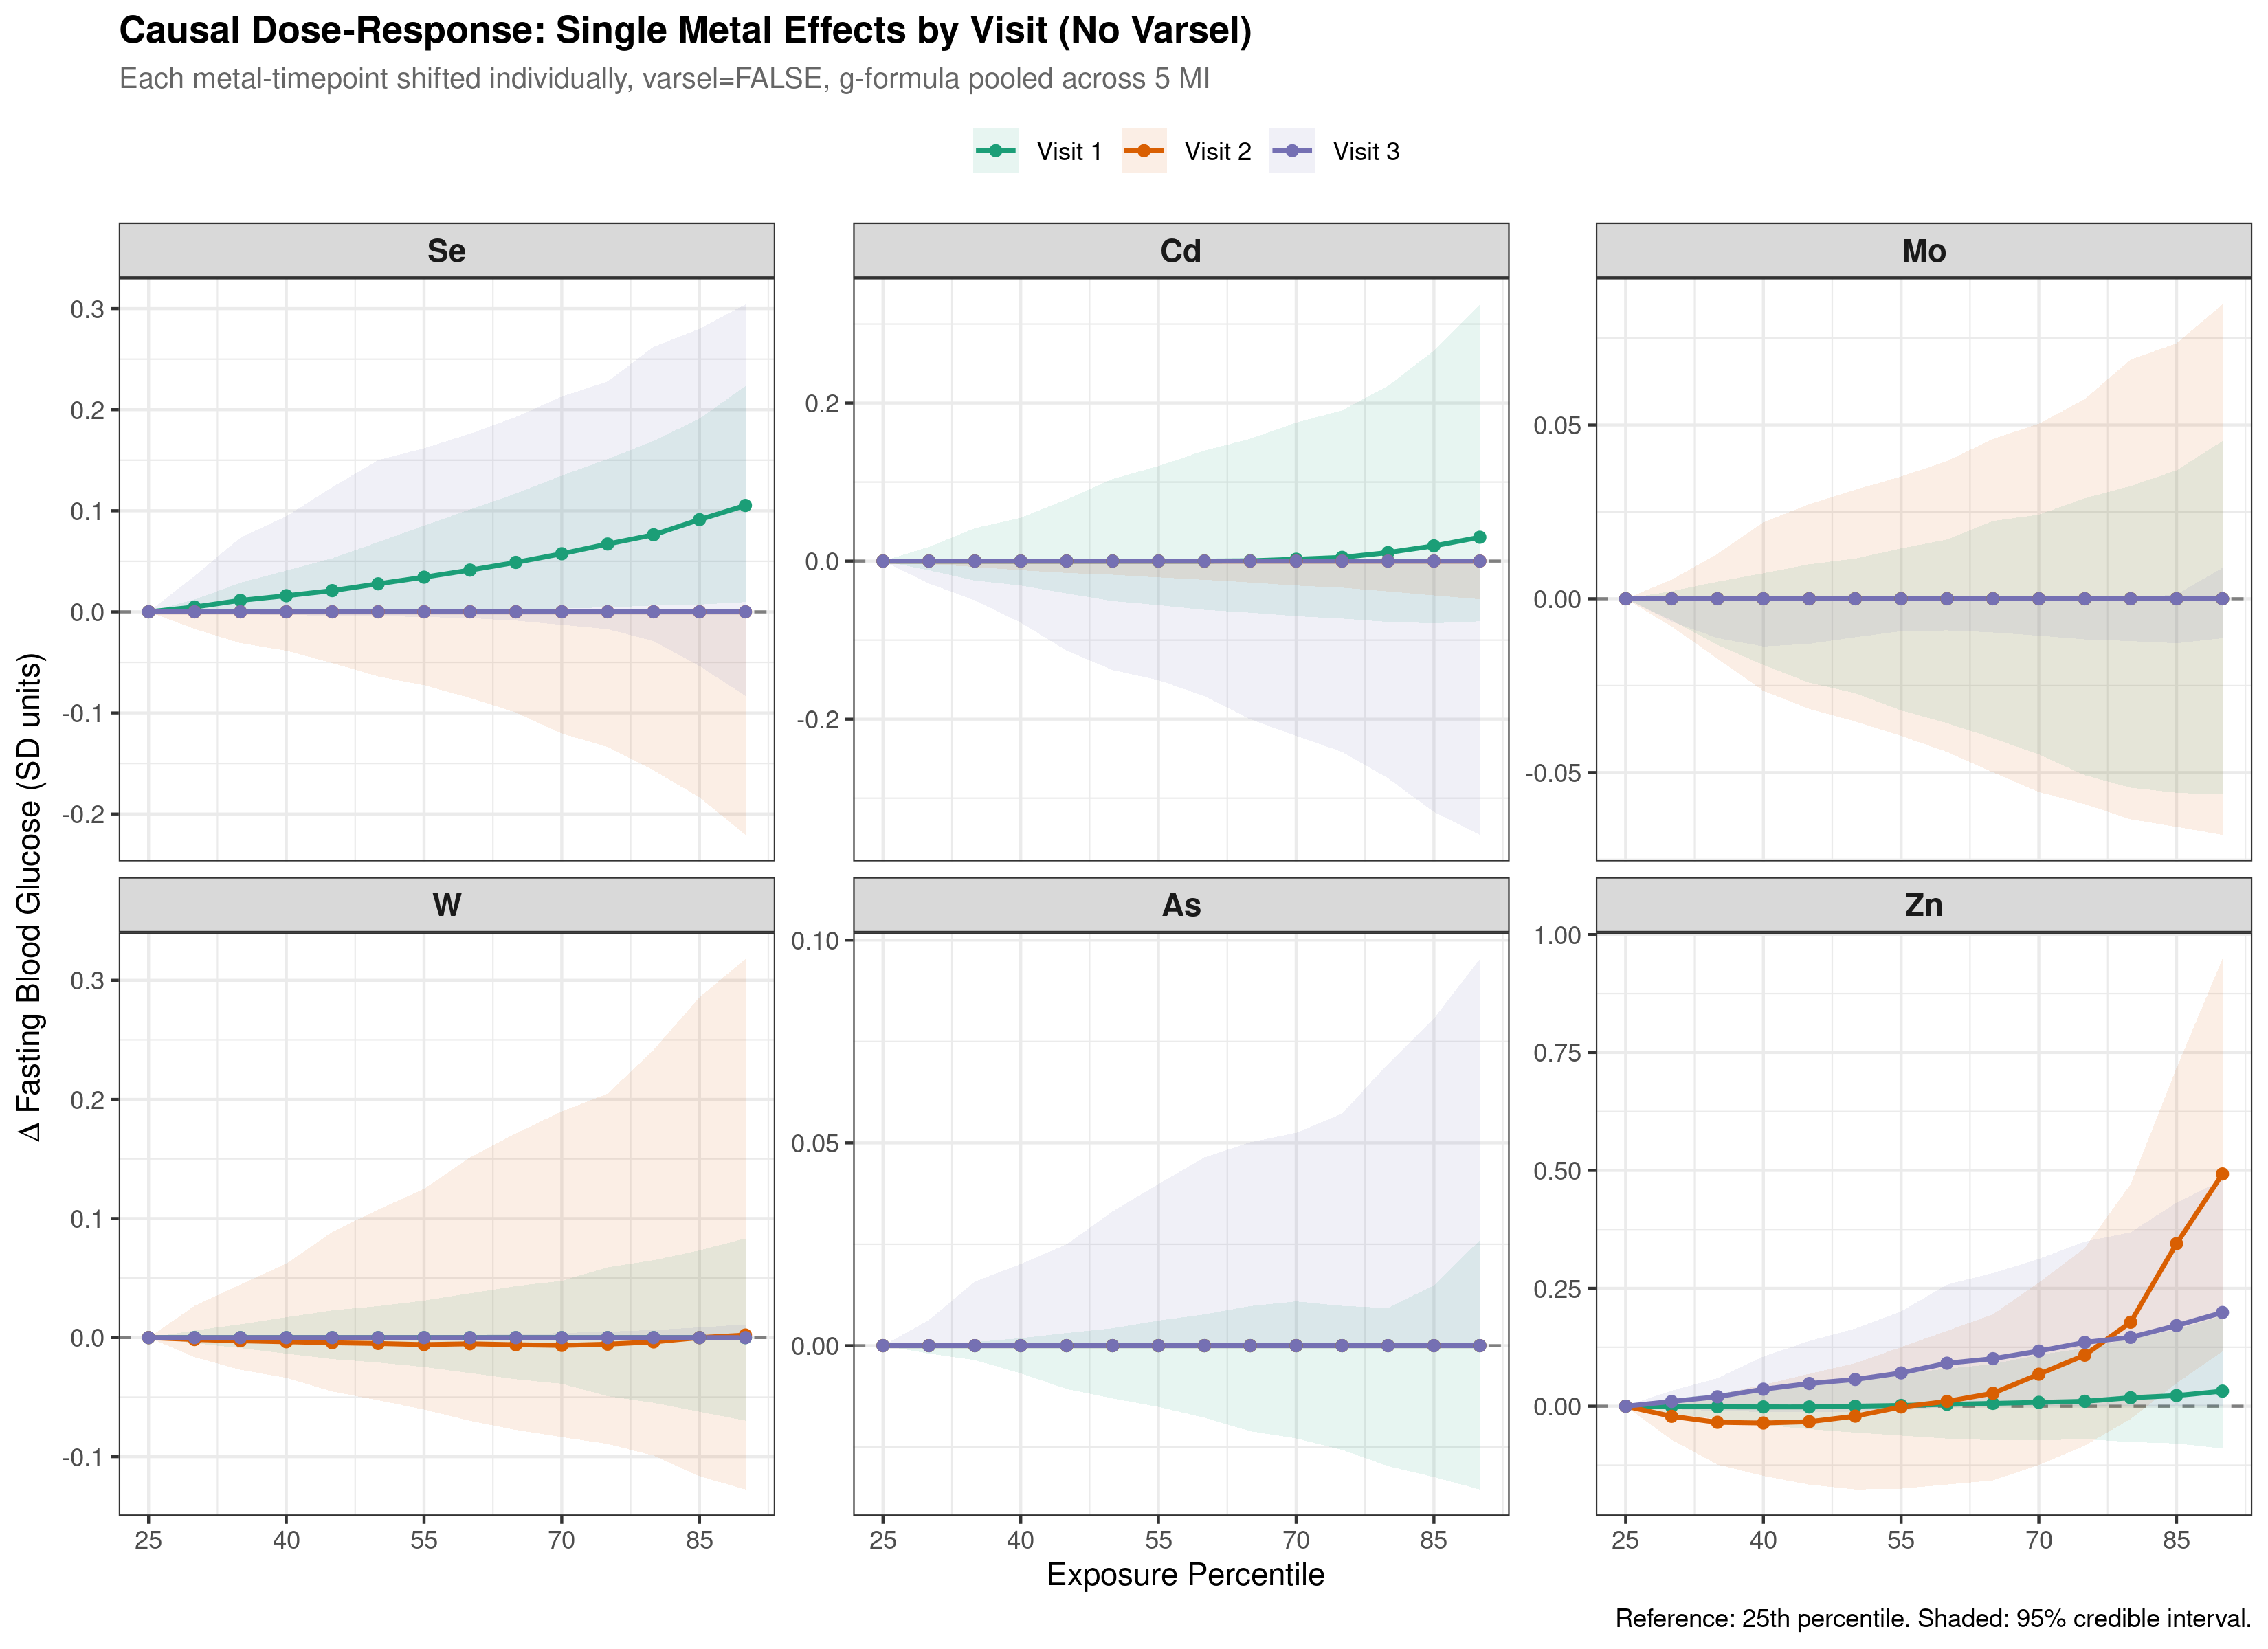
\includegraphics[width=0.85\textwidth]{figures/fig_permetal_nodm.png}
\caption{Per-metal dose-response curves, excluding baseline diabetes ($n = 414$).}
\label{fig:supp-permetal-nodm}
\end{figure}

\begin{figure}[h]
\centering
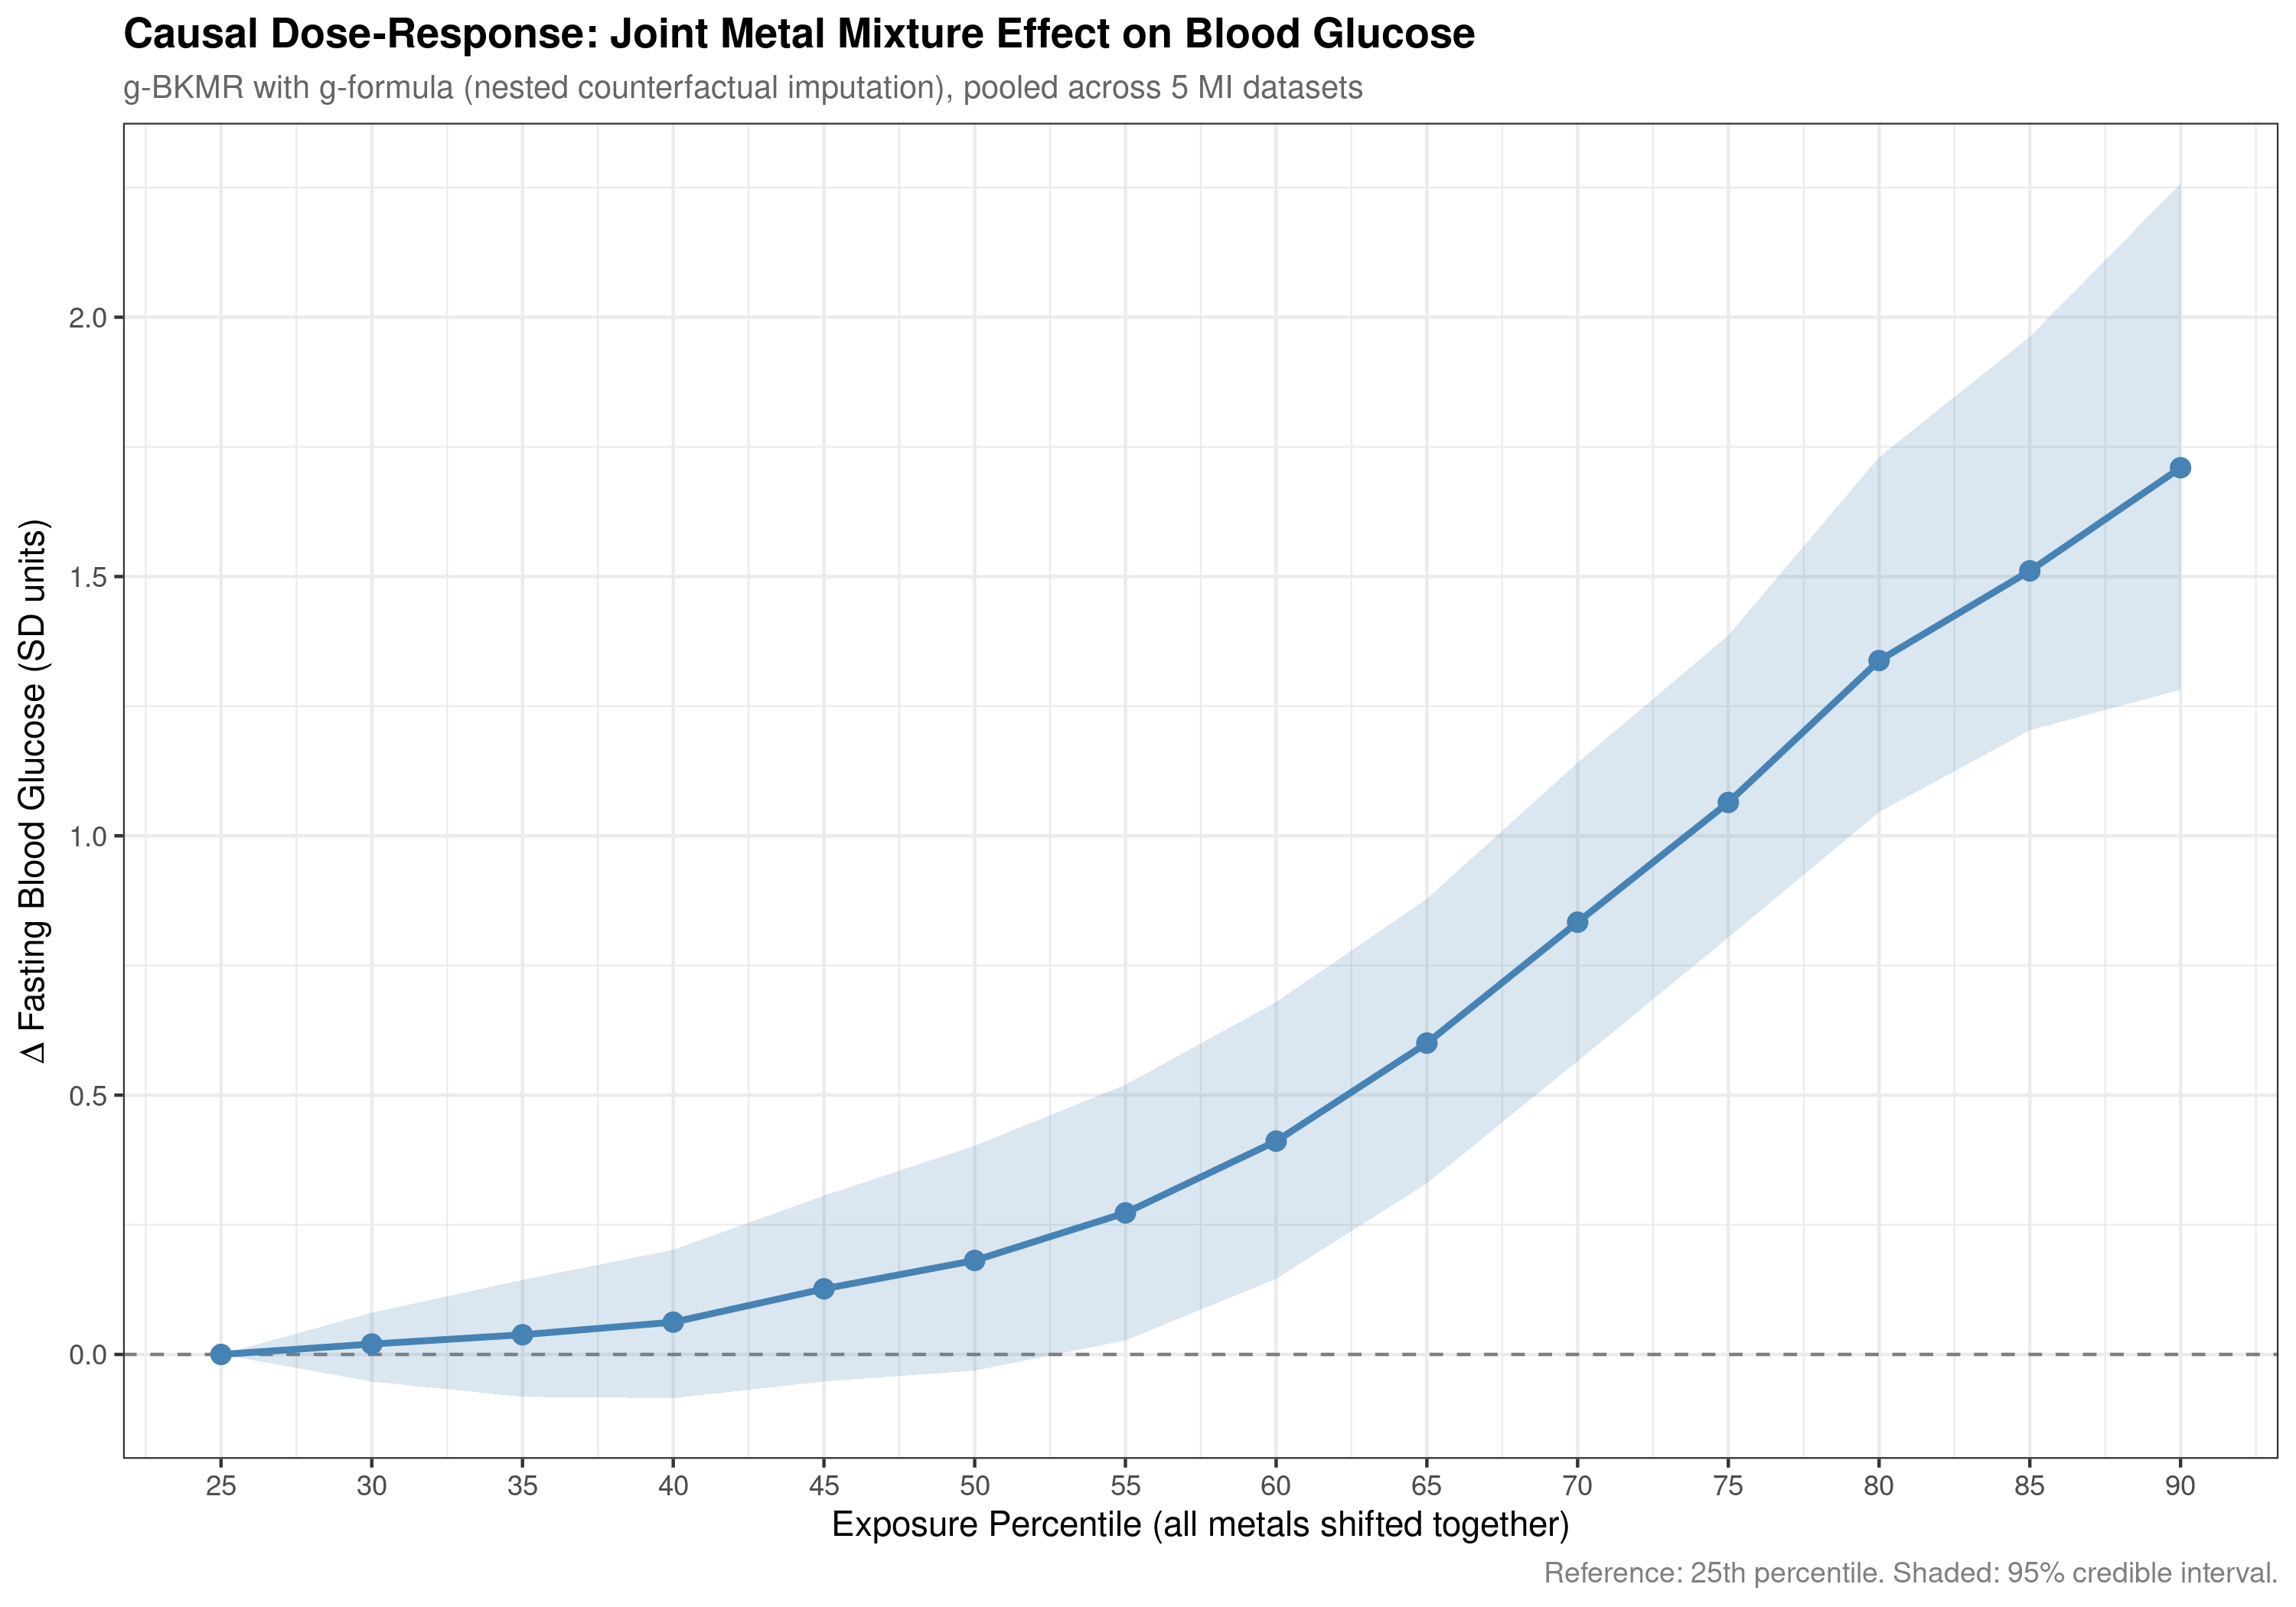
\includegraphics[width=0.85\textwidth]{figures/fig_dr_packyears.png}
\caption{Sensitivity: joint dose-response after additionally adjusting for baseline pack-years ($n = 679$).}
\label{fig:supp-dr-ppy}
\end{figure}

\begin{figure}[h]
\centering
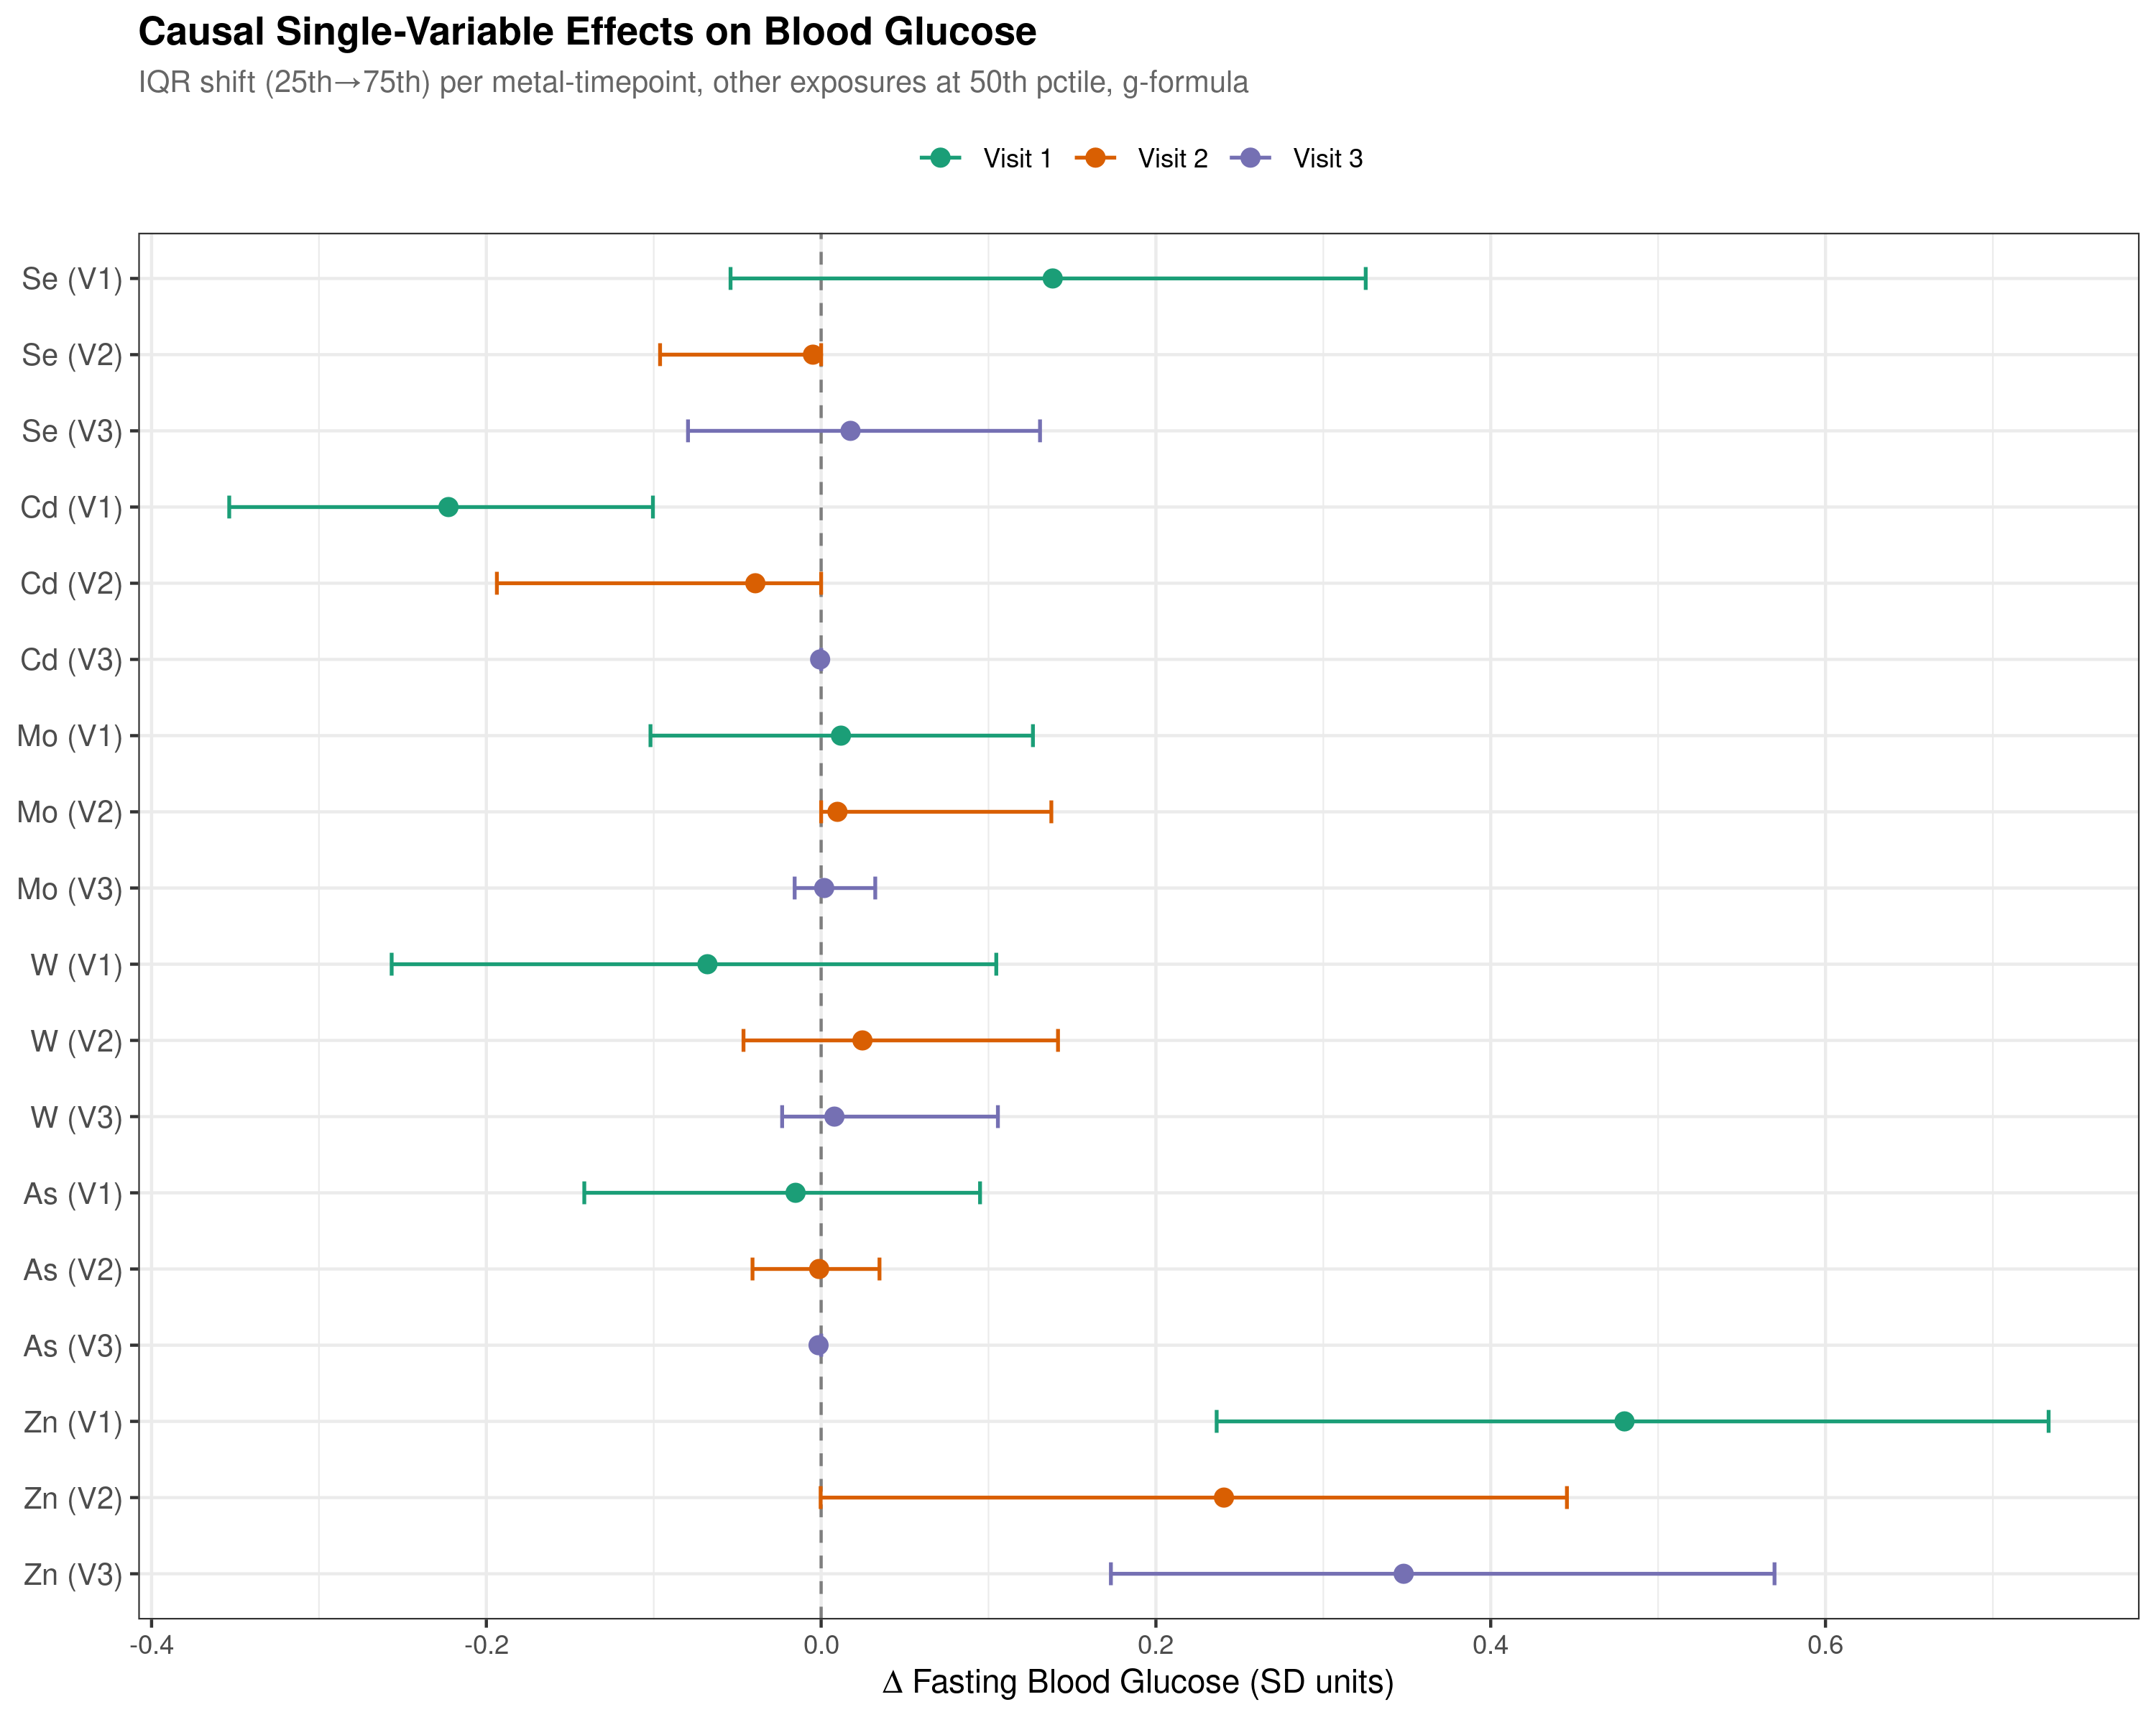
\includegraphics[width=0.85\textwidth]{figures/fig_forest_packyears.png}
\caption{Sensitivity: single-variable causal effects after additionally adjusting for baseline pack-years ($n = 679$).}
\label{fig:supp-forest-ppy}
\end{figure}

\begin{figure}[h]
\centering
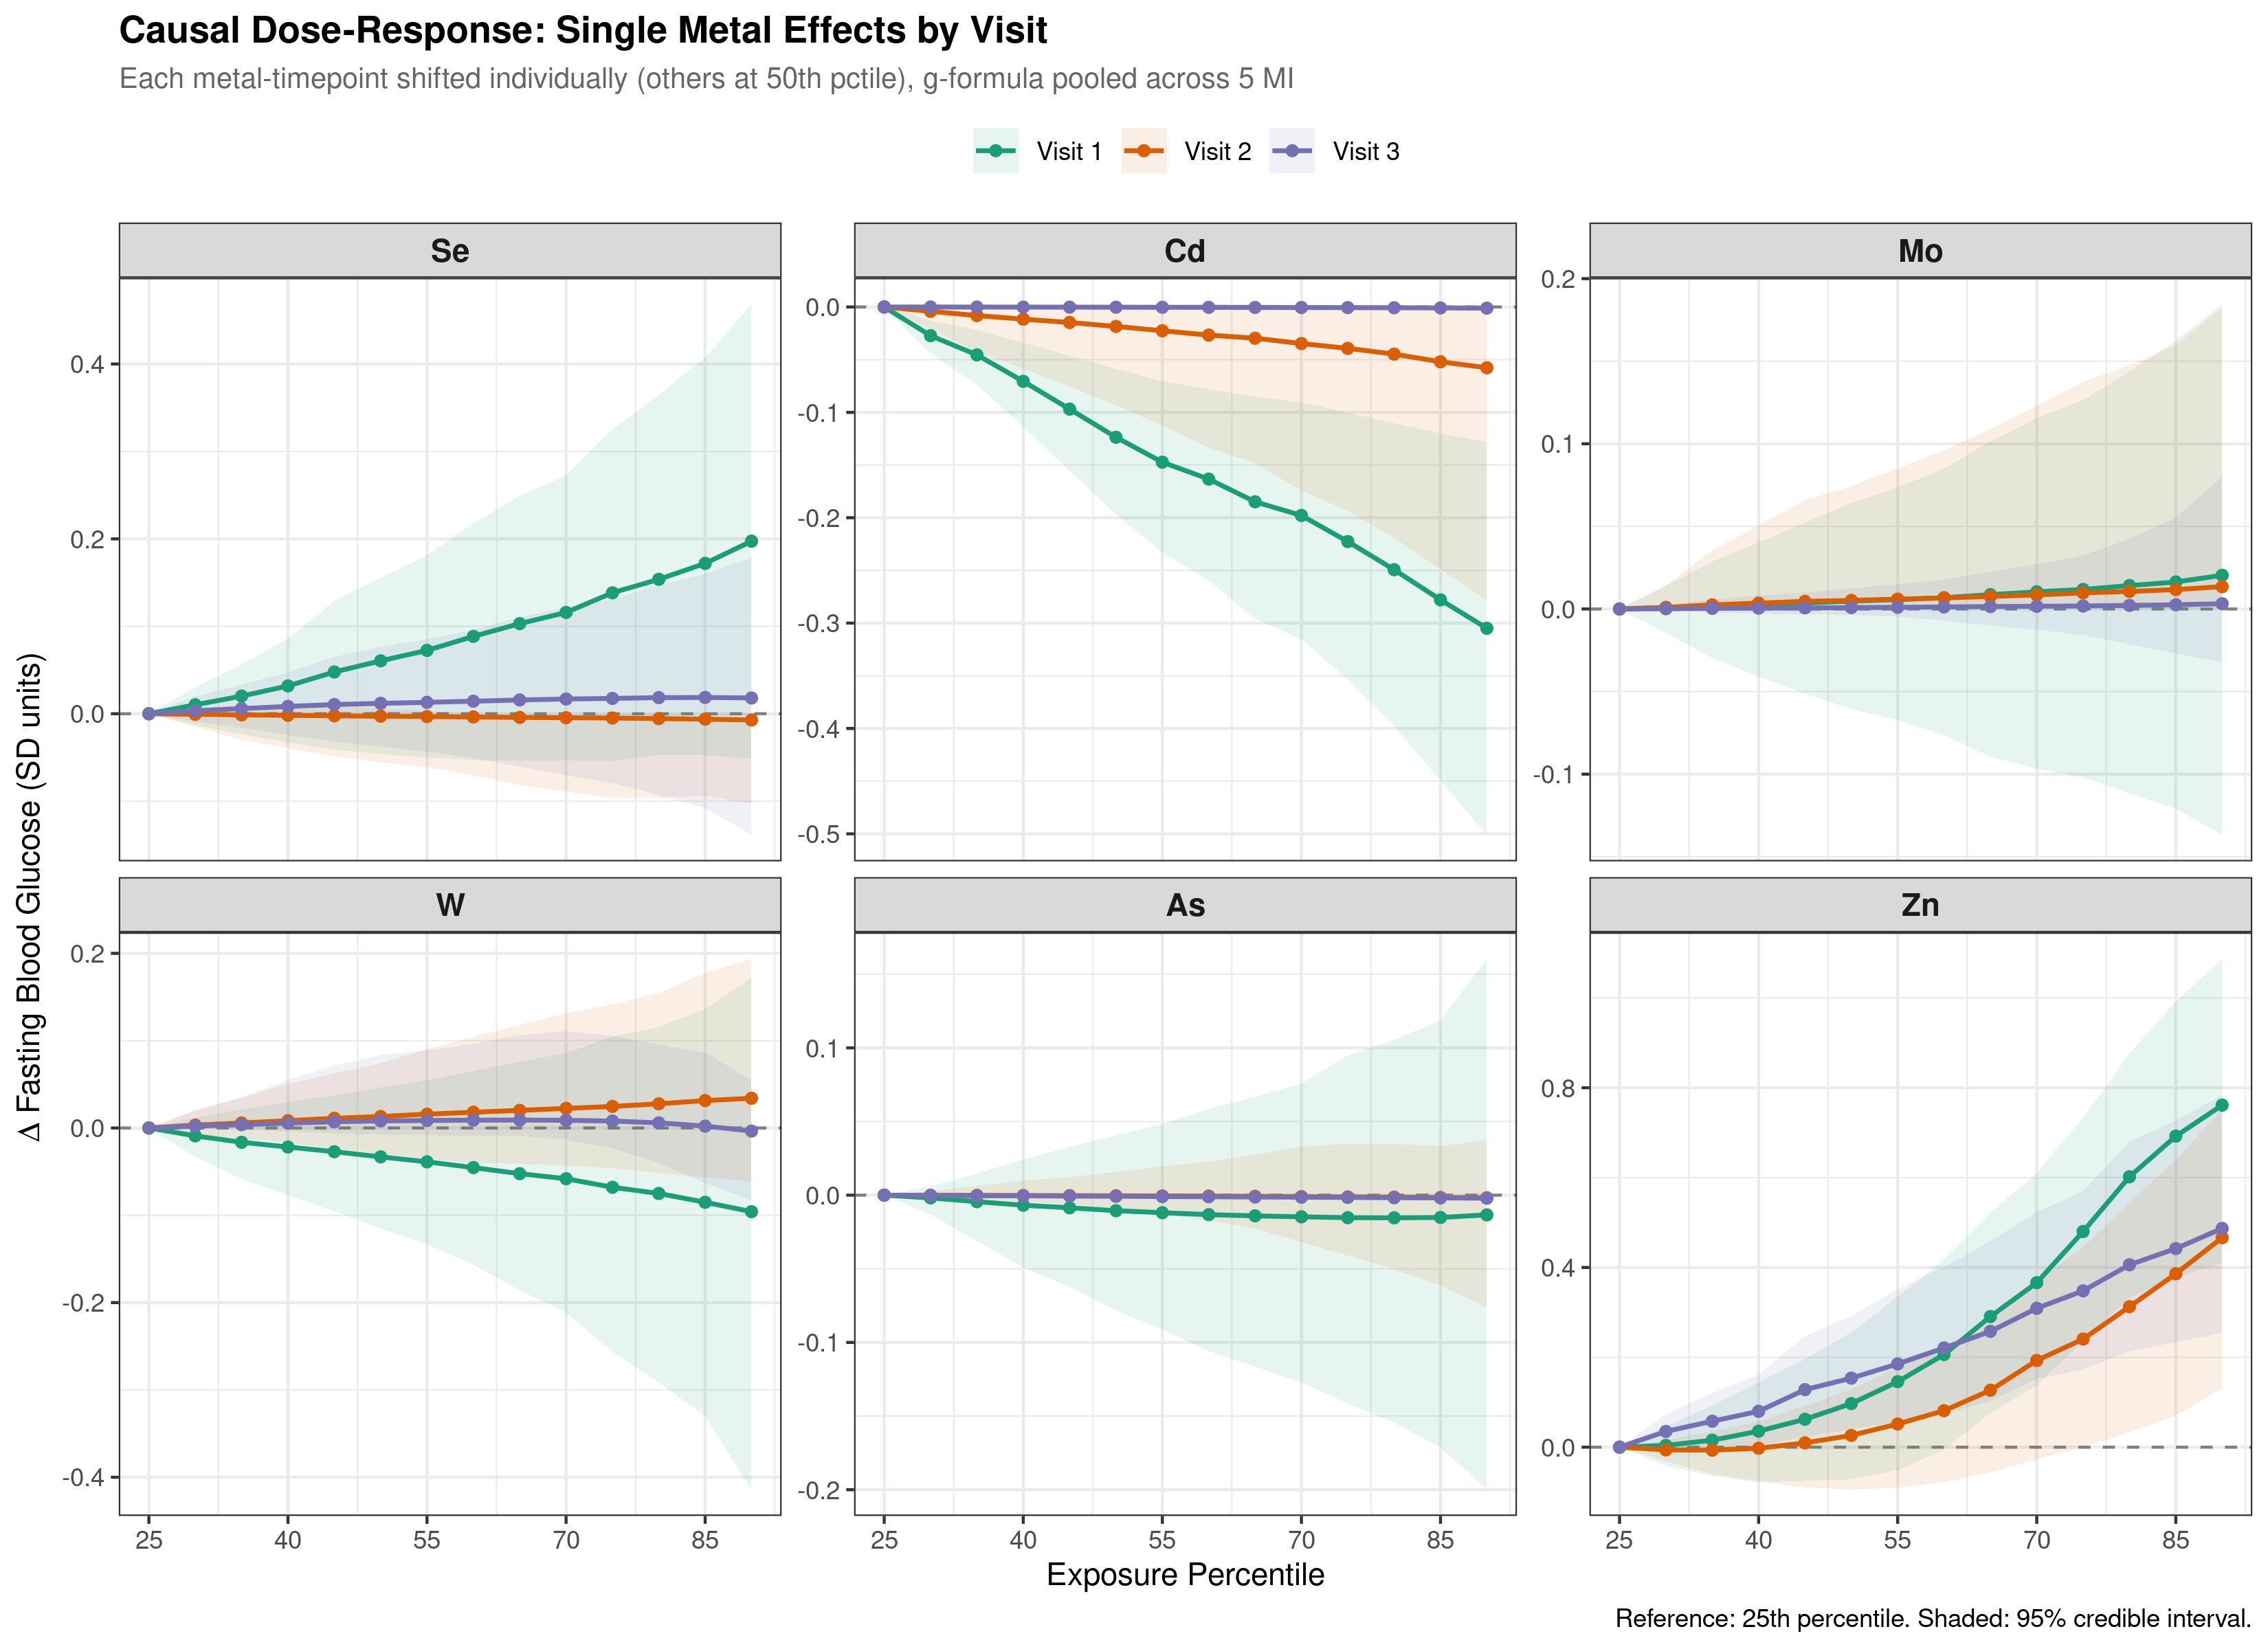
\includegraphics[width=0.85\textwidth]{figures/fig_permetal_packyears.png}
\caption{Sensitivity: per-metal dose-response curves after additionally adjusting for baseline pack-years ($n = 679$).}
\label{fig:supp-permetal-ppy}
\end{figure}

\end{document}
